\documentclass[11pt,a4paper]{article}

% ---------------------------------------------------------------------
%  TFPT --- Introduction / status assessment (English, with visualisations)
%  Comparison: previous state (tfpt-45, Papers 1-7) vs. the compiler closure
% ---------------------------------------------------------------------
\usepackage[T1]{fontenc}
\usepackage[utf8]{inputenc}
\usepackage[english]{babel}
\usepackage{lmodern}
\usepackage[a4paper,margin=2.3cm]{geometry}
\usepackage{amsmath,amssymb,amsthm}
\usepackage{booktabs}
\usepackage{tabularx}
\usepackage{multirow}
\usepackage{enumitem}
\usepackage{xcolor}
\usepackage{tikz}
\usetikzlibrary{positioning,arrows.meta,fit,backgrounds,calc,shapes.geometric,shapes.misc}
\usepackage[most]{tcolorbox}
\usepackage{microtype}
\usepackage{needspace}
\usepackage[hidelinks,colorlinks=true,linkcolor=blue!55!black,urlcolor=blue!55!black]{hyperref}

% ---- colours / boxes ----
\definecolor{tfblue}{HTML}{1F4E79}
\definecolor{tfgreen}{HTML}{1E7B45}
\definecolor{tfred}{HTML}{9B2226}
\definecolor{tfgold}{HTML}{B8860B}
\definecolor{tfgray}{HTML}{555555}

\newtcolorbox{keybox}[1][]{enhanced,breakable,colback=tfblue!5!white,colframe=tfblue,
  fonttitle=\bfseries,coltitle=white,title={#1},left=2mm,right=2mm,top=1mm,bottom=1mm}
\newtcolorbox{winbox}[1][]{enhanced,breakable,colback=tfgreen!6!white,colframe=tfgreen!75!black,
  fonttitle=\bfseries,coltitle=white,title={#1},left=2mm,right=2mm,top=1mm,bottom=1mm}
\newtcolorbox{gapbox}[1][]{enhanced,breakable,colback=tfred!5!white,colframe=tfred!80!black,
  fonttitle=\bfseries,coltitle=white,title={#1},left=2mm,right=2mm,top=1mm,bottom=1mm}

% ---- status markers ----
% --- status markers: refined six-grade system ---
\newcommand{\tI}{{\small\textcolor{tfgreen}{\textbf{[I]}}}}          % exact identity
\newcommand{\tL}{{\small\textcolor{tfblue}{\textbf{[L]}}}}           % Lie / lattice theorem
\newcommand{\tF}{{\small\textcolor{tfgreen!45!black}{\textbf{[F]}}}} % formalised (Lean / script)
\newcommand{\tN}{{\small\textcolor{tfgreen}{\textbf{[N]}}}}          % numerical fixed point
\newcommand{\tP}{{\small\textcolor{tfgold}{\textbf{[P]}}}}           % physical / conditional (under hypotheses)
\newcommand{\tA}{{\small\textcolor{tfred}{\textbf{[A]}}}}            % axiom / open
% compact, self-illustrating marker legend to place under every marker-bearing table
\newcommand{\markerkey}{\par\vspace{1.5pt}\noindent{\scriptsize\itshape\textcolor{black!58}{Marker key:\ \tI~exact identity\,$\cdot$\,\tL~Lie/lattice theorem\,$\cdot$\,\tF~formalised\,$\cdot$\,\tN~numerical fixed point\,$\cdot$\,\tP~physical/conditional\,$\cdot$\,\tA~axiom\,/\,open.}}\par\vspace{2pt}}
% inline reference to the script that machine-checks a claim (see verification/)
\newcommand{\veri}[1]{\,{\footnotesize\textcolor{tfblue!70!black}{[\,\texttt{verification/#1}\,]}}}

% ---- short macros ----
\newcommand{\cthree}{c_3}
\newcommand{\gcar}{g_{\mathrm{car}}}
\newcommand{\Nfam}{N_{\mathrm{fam}}}
\newcommand{\phiz}{\varphi_0^{\mathrm{ret}}}
\newcommand{\Oadm}{\Omega_{\mathrm{adm}}}
\newcommand{\ainv}{\alpha^{-1}}
\newcommand{\Mbar}{\bar M_{\mathrm{Pl}}}
\newcommand{\Mpl}{M_{\mathrm{Pl}}}
\newcommand{\Z}{\mathbb{Z}}
\newcommand{\PP}{\mathbb{P}}

\setlist{itemsep=2pt,topsep=3pt}
\newcolumntype{Y}{>{\raggedright\arraybackslash}X}
\emergencystretch=2.5em

\title{\vspace{-1.2cm}\textbf{The Compiler Closure of TFPT}\\[2mm]
\large What concretely simplifies, reduces and closes relative to the\\
seven original papers --- a status assessment and reading guide}
\author{}
\date{\today}

\begin{document}
\maketitle
\vspace{-0.8cm}

\begin{keybox}[In one sentence]
The theory tips from ``many sectors with surprising hits'' (the state of Papers 1--7) to
``\emph{one small discrete compiler generates those sectors}'': $E_8$ --- which in v4.5 appeared only
\emph{peripherally} (the orbit cascade for scale ordering) --- is now \emph{built} from two TFPT atoms and
moved to the centre; the flavor matrix, the fine-structure constant and the scale grammar follow as
\emph{fixed points} from exactly two inputs $\cthree=\tfrac1{8\pi}$ and $\gcar=5$.
\end{keybox}

\begin{keybox}[The TFPT document set --- what is treated where]
\textbf{Plain language:} TFPT is a small discrete compiler. Two inputs --- the seam constant
$\cthree=\tfrac1{8\pi}$ and the carrier rank $\gcar=5$ --- build $D_5\oplus A_3+\mu_4\Rightarrow E_8$ and
read off the Standard Model, the constants and the scale grammar. The development is \textbf{five short
documents plus Appendix~H}, best read in order (this is the entry point; a detailed map is in \S\ref{sec:docmap}):
\begin{enumerate}[leftmargin=1.7em,itemsep=1pt]
\item \texttt{introduction} --- reading guide, compiler closure, paper-by-paper comparison, predictions, the dependency DAG and proof ledger.
\item \texttt{tfpt\_1\_architecture\_e8} --- the two axioms, the derivation map, the EM fixed point $\ainv$, the $D_5\oplus A_3+\mu_4\Rightarrow E_8$ construction.
\item \texttt{tfpt\_2\_standard\_model} --- the SM in one $\varphi_0$-ladder formula, flavor from parabolic transport, the worked closures, and gravity/QG as the seam response.
\item \texttt{tfpt\_3\_e8\_audit\_bootstrap} --- the seven $E_8$ slices as an audit raster, the cascade bridge, the M\"obius bootstrap.
\item \texttt{tfpt\_4\_frontier} --- honest status of $\eta_B$, $m_p/m_e$, Koide, dark matter, full QG.
\item[H.] \texttt{tfpt\_horizon\_readouts} --- \textbf{Appendix~H} (unit-system reframe, \emph{not} new physics): one seam constant as the universal horizon thermal code.
\item[O.] \texttt{origin\_theory} --- \textbf{Origin Theory}: why no free fundamental number remains. The $(\gcar,\Nfam){=}(5,3)$ skeleton, the triply-forced $8$ (geometry $=$ lattice $=$ gravity), the order-$30$ Coxeter cycle, one boundary transport for flavor and horizon, and the gapped \emph{unique attractor}. \tI/\tL\ core ($\mathtt{v53}$--$\mathtt{v56}$) plus one honestly-typed \tP\ cyclic interpretation.
\end{enumerate}
\textbf{You are reading document \#1.}
\end{keybox}

\tableofcontents

\noindent\textbf{Reading the markers (refined).} The former overloaded ``[M]'' is split into the grade it
actually carries, so a reviewer can see at a glance which claims are exact, which are formal, and which are
conditional:
\tI\ \emph{exact identity} (e.g.\ $240=16\cdot5\cdot3$);
\tL\ \emph{Lie/lattice theorem} (e.g.\ $D_5{\oplus}A_3{+}\mu_4{=}E_8$);
\tF\ \emph{formalised} (Lean- or script-verified);
\tN\ \emph{numerical fixed point} (reproduced, stable);
\tP\ \emph{physical/conditional} (follows under named hypotheses);
\tA\ \emph{axiom or open}.

\begin{center}
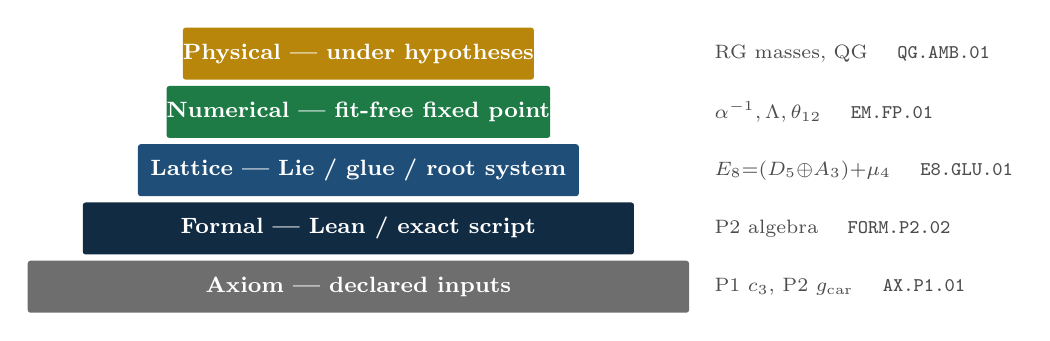
\begin{tikzpicture}[font=\footnotesize,
  band/.style={rounded corners=1pt,inner sep=0pt,minimum height=6.6mm,text=white,font=\footnotesize\bfseries,align=center},
  tag/.style={anchor=west,font=\scriptsize,black!70}]
  \node[band,fill=tfgray!85,   minimum width=84mm] (b0) at (0,0.00) {Axiom --- declared inputs};
  \node[band,fill=tfblue!55!black,minimum width=70mm] (b1) at (0,0.74) {Formal --- Lean / exact script};
  \node[band,fill=tfblue,      minimum width=56mm] (b2) at (0,1.48) {Lattice --- Lie / glue / root system};
  \node[band,fill=tfgreen,     minimum width=42mm] (b3) at (0,2.22) {Numerical --- fit-free fixed point};
  \node[band,fill=tfgold,      minimum width=28mm] (b4) at (0,2.96) {Physical --- under hypotheses};
  \node[tag] at (44mm,0.00) {P1 $\cthree$, P2 $\gcar$ \quad\texttt{AX.P1.01}};
  \node[tag] at (44mm,0.74) {P2 algebra \quad\texttt{FORM.P2.02}};
  \node[tag] at (44mm,1.48) {$E_8{=}(D_5{\oplus}A_3){+}\mu_4$ \quad\texttt{E8.GLU.01}};
  \node[tag] at (44mm,2.22) {$\ainv,\Lambda,\theta_{12}$ \quad\texttt{EM.FP.01}};
  \node[tag] at (44mm,2.96) {RG masses, QG \quad\texttt{QG.AMB.01}};
\end{tikzpicture}
\end{center}
\noindent\emph{The claim stack} (bottom $=$ most certain/fewest, top $=$ conditional). Each claim sits on
exactly one level; the bottom two are inputs, the middle two are proved/reproduced, only the top is
conditional. The single source of truth for which claim sits where is
\texttt{verification/status\_ledger.csv} (Fig.~\ref{fig:statusheat}).

\smallskip
\noindent\textbf{No-free-pattern rule.} To keep the structure from drowning in decorative coincidences, an
identity enters the \emph{main text} only if it (1) is a necessary step in a derivation, (2) kills an
alternative, (3) is ablation-relevant, (4) links two previously independent modules, or (5) is
experimentally tested. Everything else is explicitly demoted to an \emph{audit fingerprint} \tI\ (clearly
boxed as such) --- so the load-bearing beams stay visible and the ornament never gets promoted to spine.

\noindent\textbf{Admissible-invariant classes (the harder filter).} Sharper still: a \emph{load-bearing}
integer may only come from one of seven typed sources --- (i) a symmetric function $e_k(a)$ of the anchor
$a=(1,1,2)$; (ii) a power sum $p_n(a)$ or difference $p_{n+1}{-}p_n$; (iii) a determinant, spectrum, Smith
normal form or trace of $(R,Q,K,L)$; (iv) an anchor quadratic form $u^\top M v$ with $u,v\in\{\mathbf1,a\}$;
(v) a Pl\"ucker coordinate of the anchor plane $\langle\mathbf1,a\rangle$; (vi) an $E_8$ Casimir degree or
branching block; (vii) a pre-registered experimental observable. Anything else is an audit fingerprint or a
frontier item, never spine. This is what converts TFPT from \emph{pattern hunting} (``look, another number'')
into a typed compiler: \emph{fewer admissible kinds of explanation}, not more matches.

\begin{keybox}[Reviewer path (read in this order; the rest is support)]
\begin{enumerate}[leftmargin=1.7em,itemsep=1pt]
\item the architecture: the two axioms $\{\cthree,\gcar\}$ and the two-engine picture (\S\ref{sec:docmap}, the figures);
\item the $E_8$ glue $E_8{=}(D_5{\oplus}A_3){+}\mu_4$ --- document~1, Part~II, machine-checked (\texttt{verification/v1\_e8\_glue.py});
\item the $\alpha^{-1}$ fixed point plus ablation (\texttt{v3\_em\_alpha.py});
\item the \textbf{single status ledger} \texttt{verification/status\_ledger.csv} --- the source of truth for every claim's grade, location, dependency and script;
\item the honest frontier list (document~4).
\end{enumerate}
Everything carries a claim ID (e.g.\ \texttt{E8.GLU.01}, \texttt{EM.FP.01}) that resolves to a row of the
ledger. \textbf{If the text and the ledger ever disagree, the ledger wins.}
\end{keybox}

% =====================================================================
\section{What this is about: the jump in construction principle}\label{sec:docmap}
% =====================================================================

\begin{keybox}[In plain words --- what we found, and why it matters]
\textbf{What we found.} The older version of the theory already reproduced dozens of real numbers of
physics (particle masses, the fine-structure constant, dark-energy and inflation values) from a small set
of inputs. What it could \emph{not} say was \emph{why} the same handful of small integers
($2,3,5,16,\dots$) kept reappearing in every sector. The new result closes exactly that gap: those
numbers are not separate lucky hits. A single tiny ``machine'' --- fed by just \textbf{two inputs} (a
boundary number $\tfrac1{8\pi}$ and a five-slot carrier) --- builds the exceptional symmetry $E_8$, and
$E_8$ is the unimodular ``audit hull'' that classifies the discrete Standard-Model readout: the constants,
the flavor skeleton and the gravity/cosmology regime are then read off by projection and boundary dressing
(not ``printed'' for free --- where a scheme or analytic interface is needed, it is named).

\smallskip
\textbf{How this drastically simplifies the theory.} Instead of seven separate derivations that happen to
share numbers, there is now \emph{one generator and a handful of corollaries}. Roughly $250$ pages of
sector-by-sector work collapse to ``two inputs $+$ one machine''; the number of independent structural
assumptions drops to \textbf{two}.

\smallskip
\textbf{How plausible it is.} A theory becomes more believable when it \emph{explains more from less}.
Here the two inputs are even \emph{over-determined}: the machine reproduces the very two numbers it started
from (the dashed loop below), so there is \emph{no free dial left to tune}. The only genuinely free,
continuous ingredient that remains is the number $\pi$.
\end{keybox}

\begin{center}
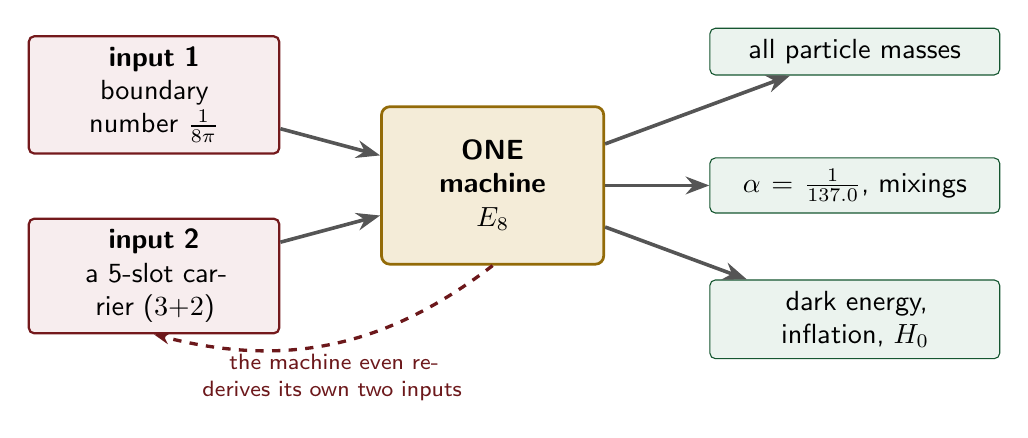
\begin{tikzpicture}[font=\sffamily,
  knob/.style={rectangle,rounded corners=2pt,draw=tfred!75!black,fill=tfred!8,thick,align=center,inner sep=4pt,text width=29mm,minimum height=12mm},
  machine/.style={rectangle,rounded corners=3pt,draw=tfgold!80!black,fill=tfgold!16,line width=1pt,align=center,inner sep=6pt,text width=24mm,minimum height=20mm},
  outp/.style={rectangle,rounded corners=2pt,draw=tfgreen!70!black,fill=tfgreen!9,align=center,inner sep=4pt,text width=34mm},
  fat/.style={-{Stealth[length=3mm]},line width=1.3pt,tfgray}]
  \node[knob] (k1) at (0,1.15) {\textbf{input 1}\\boundary number $\tfrac1{8\pi}$};
  \node[knob] (k2) at (0,-1.15) {\textbf{input 2}\\a 5-slot carrier ($3{+}2$)};
  \node[machine] (m) at (4.3,0) {\textbf{ONE}\\\textbf{machine}\\$E_8$};
  \node[outp] (o1) at (8.9,1.7)  {all particle masses};
  \node[outp] (o2) at (8.9,0.0)  {$\alpha=\tfrac1{137.0}$, mixings};
  \node[outp] (o3) at (8.9,-1.7) {dark energy, inflation, $H_0$};
  \draw[fat] (k1) -- (m); \draw[fat] (k2) -- (m);
  \draw[fat] (m) -- (o1); \draw[fat] (m) -- (o2); \draw[fat] (m) -- (o3);
  \draw[-{Stealth[length=2mm]},very thick,dashed,tfred!70!black] (m.south) to[bend left=26]
     node[below,font=\footnotesize\sffamily,text width=46mm,align=center]{the machine even re-derives its own two inputs} (k2.south);
\end{tikzpicture}\\[4pt]
{\small\itshape Two numbers go in on the left; the discrete Standard-Model core, the dimensionless
constants and several scale readouts come out on the right --- and the dashed loop is the point: the
machine reproduces the very two numbers it started from, so the discrete core is \emph{overdetermined}
rather than fitted. (Dimensionful EW/QCD masses, the full quantum-gravity measure and the frontier items
stay typed-open --- see the status ledger.)}
\end{center}

\medskip
The seven original papers (\texttt{tfpt-45}, Papers 1--7) deliver a long chain of physical closures:
boundary kernel $\to$ carrier $\to$ Standard-Model packet $\to$ EM fixed point $\to$ flavor transport
$\to$ admissibility/strong CP $\to$ geometric gravity/metrology $\to$ cosmology/CMB. Each stage stands on
its own and hits a remarkable number of values. What was missing was a \emph{meta-statement} explaining
\emph{why} so many independent sectors use the same small stock of numbers
($2,3,5,16,40,41,48,240,248$).

\begin{center}
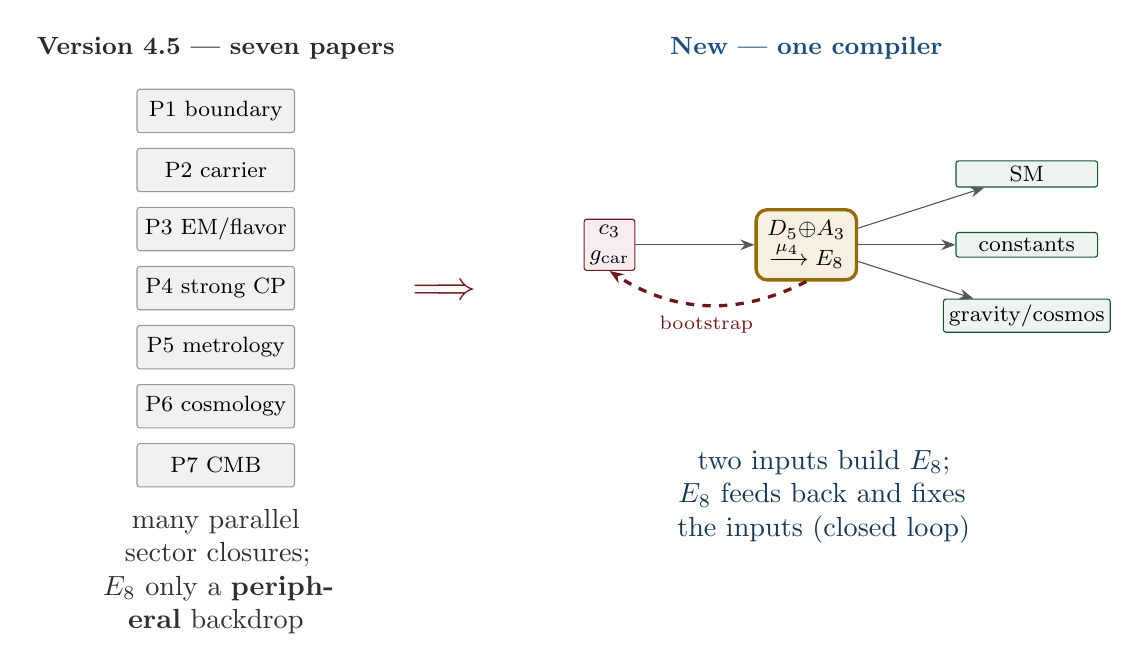
\begin{tikzpicture}[font=\footnotesize,
  pap/.style={rectangle,rounded corners=1pt,draw=tfgray!60,fill=tfgray!8,align=center,inner sep=2pt,minimum width=20mm,minimum height=5.5mm},
  cmp/.style={rectangle,rounded corners,draw=tfgold!80!black,fill=tfgold!12,very thick,align=center,inner sep=4pt},
  ob/.style={rectangle,rounded corners=1pt,draw=tfgreen!70!black,fill=tfgreen!8,align=center,inner sep=2pt,minimum width=18mm},
  ar/.style={-{Stealth[length=1.8mm]},tfgray}]
% ---- left panel: v4.5 ----
\node[font=\bfseries\small,tfgray!50!black] at (-4.3,3.1) {Version 4.5 --- seven papers};
\foreach \y/\lab in {2.3/{P1 boundary},1.55/{P2 carrier},0.8/{P3 EM/flavor},0.05/{P4 strong CP},-0.7/{P5 metrology},-1.45/{P6 cosmology},-2.2/{P7 CMB}}{
  \node[pap] at (-4.3,\y) {\lab};}
\node[font=\itshape,tfgray!55!black,align=center,text width=34mm] at (-4.3,-3.55) {\emph{many parallel sector closures;\\ $E_8$ only a \textbf{peripheral} backdrop}};
% ---- arrow ----
\node[font=\Large\bfseries,tfred!75!black] at (-1.4,0) {$\Longrightarrow$};
% ---- right panel: compiler ----
\node[font=\bfseries\small,tfblue] at (3.2,3.1) {New --- one compiler};
\node[rectangle,rounded corners=1pt,draw=tfred!80!black,fill=tfred!8,align=center,inner sep=2pt] (in) at (0.7,0.6) {$\cthree$\\$\gcar$};
\node[cmp] (c) at (3.2,0.6) {$D_5{\oplus}A_3$\\$\xrightarrow{\mu_4}E_8$};
\node[ob] (o1) at (6.0,1.5) {SM};
\node[ob] (o2) at (6.0,0.6) {constants};
\node[ob] (o3) at (6.0,-0.3) {gravity/cosmos};
\draw[ar] (in)--(c); \draw[ar] (c)--(o1); \draw[ar] (c)--(o2); \draw[ar] (c)--(o3);
\draw[-{Stealth[length=1.8mm]},very thick,dashed,tfred!70!black] (c.south) to[bend left=30] node[below,font=\scriptsize]{bootstrap} (in.south);
\node[font=\itshape,tfblue!70!black,align=center,text width=42mm] at (3.4,-2.6) {\emph{two inputs build $E_8$; $E_8$ feeds back and fixes the inputs (closed loop)}};
\end{tikzpicture}
\end{center}

\noindent\textbf{The difference in one picture.} v4.5 is a \emph{stack of seven independent closures} that
happen to share numbers, with $E_8$ assumed in the background. The new approach is \emph{one discrete
compiler}: two inputs build $E_8$, $E_8$ outputs the sectors, \emph{and} $E_8$ feeds back to fix the two
inputs (the red loop). What were seven parallel results become one generator with corollaries; what was a
posited $E_8$ becomes a constructed-and-self-checking closure.

\begin{keybox}[Sharper still: one anchor $a=(1,1,2)$, and $E_8$ as a \emph{compiler hull} \tI/\tL]
The two axioms are not even independent: they are the \emph{elementary symmetric polynomials} of the
single parabolic anchor $a=(1,1,2)$ (the exponents-at-infinity / splitting type $\mathcal O(-2)\oplus\mathcal O(-1)^2$):
\[
  e_1(a)=4=|\mu_4|,\qquad e_2(a)=5=\gcar,\qquad e_3(a)=2=|\Z_2|,\qquad
  \cthree=\frac1{2e_1(a)\pi}=\frac1{8\pi}.
\]
Its \emph{power sums} $p_n(a)=1^n{+}1^n{+}2^n=2{+}2^n$ generate the big Lie data directly:
$p_1{=}4{=}|\mu_4|$, $p_2{=}6{=}|R^+(A_3)|$, $p_3{=}10{=}\mathcal A_\Lambda$, and
\[
  |R(E_8)|=p_1p_2p_3=240,\quad \dim E_8=p_1p_2p_3+(p_4-p_3)=248,\quad p_4-p_3=8=\operatorname{rank}E_8,
\]
with the binary ladder $p_{n+1}-p_n=2^n$. So the inputs collapse from $\{\cthree,\gcar\}$ to
$\boxed{\,a=(1,1,2)\ \text{plus}\ \pi\,}$. \veri{v23\_anchor\_generator.py}
\smallskip\\
\noindent\emph{And $a$ is itself half-forced} (\tL/\tP): on $\mathbb P^1$ every bundle splits
(Birkhoff--Grothendieck), so once $|\mu_4|=4$, $\Nfam=3$, $\deg E=-4$ are set, the three positive
anti-degrees are positive integers summing to $4$, and $4=2+1+1$ is the \emph{unique} partition into three
positive parts. The genuine remaining axiom is therefore not ``why $a=(1,1,2)$'' but ``why the carrier
$\gcar=5$ / $(|\mu_4|,\Nfam)=(4,3)$'' --- that interface (with $\cthree$) is the \tA\ input layer.
\smallskip\\
\noindent\textbf{What $E_8$ is (and is not).} In TFPT $E_8$ is \emph{not} an unbroken physical gauge group:
it is the unimodular \emph{audit / compiler hull} that classifies the admissible discrete charge and
residue structures. The Standard Model is a \emph{readout} after projection, not a direct $E_8$ gauge
theory; the Lorentz signature appears only after projection; fermions are not ``everything in the
adjoint''. This is exactly why the known no-go results against literal $E_8$ world-formulas
(Distler--Garibaldi; Coleman--Mandula) do \emph{not} bite: they constrain $E_8$ as a spacetime gauge
symmetry, which TFPT does not claim. The defensible claim is: \emph{TFPT is the unique parabolic
compilation of the anchor $a=(1,1,2)$ into the $E_8$ audit hull.}
\smallskip\\
\noindent In one line:
\[
  \boxed{\ \text{The anchor generates the syntax; the boundary generates the scale; }E_8\text{ checks the consistency.}\ }
\]
i.e.\ the discrete content (carrier $D_5\oplus A_3+\mu_4$, the operators $R,Q,K,L$) flows from
$a=(1,1,2)$; the continuous content ($c_3=\tfrac1{8\pi}$, $\varphi_0$, $\ainv$, the exponential scales) flows
from $\pi$; and $E_8$ is the unimodular \emph{checksum container}, not the world group.
\end{keybox}

That is now the case. The whole development is consolidated into \textbf{five companion documents} (plus
this introduction), organised in layers that build on one another; this introduction is the entry point
and reading guide. Each document collects the earlier notes of its layer into self-contained parts:

\begin{center}\scriptsize
\renewcommand{\arraystretch}{1.25}
\begin{tabularx}{\linewidth}{@{}p{3.6cm}Y@{}}
\toprule
\textbf{Document} & \textbf{What it contains (former notes now as parts)} \\
\midrule
\texttt{tfpt\_1\_architecture\_e8} & \textbf{Core.} The two axioms $\{\cthree,\gcar\}$, the derivation map and the EM fixed point (Part~I); the Coxeter--cyclotomic compiler $\Z_{30}{=}2{\cdot}3{\cdot}5$, the explicit $D_5{\oplus}A_3{+}\mu_4$ $E_8$ construction, the machine-checkable $E_8$ appendix and the group-level glue $(\mathrm{Spin}(10){\times}SU(4))/\Delta\Z_4$ (Part~II). \\
\texttt{tfpt\_2\_standard\_model} & \textbf{Standard Model.} The full SM in one $\phiz$-ladder formula (Part~I); the flavor block from parabolic weights and the transport theorem, H2 as a spectral selector (Part~II); the worked closures --- explicit gap, APS--Fredholm, truncation/$n_s,r$, Starobinsky $M$, derived $\theta_{12}$, quark $c$, the H2 splitting type, $\Lambda$-typing (Part~III). \\
\texttt{tfpt\_3\_e8\_audit\_bootstrap} & \textbf{$E_8$ audit \& bootstrap.} The seven $E_8$ slices as an audit raster ($E_6{\times}A_2$ reads the flavor matrix) (Part~I); the old cascade $D{=}60{-}2n$ as the same even-integer spine (Part~II); the M\"obius bootstrap --- $\gcar{=}5$ and the ``$8$'' in $\cthree$ as overdetermined fixed points, only $\pi$ irreducible (Part~III). \\
\texttt{tfpt\_4\_frontier} & \textbf{Frontier.} The honest status of $\eta_B$, $m_p/m_e$, Koide, dark matter and quantum gravity --- the genuine handle, the precision, and what is \emph{not} forced onto the ladder. \\
\texttt{tfpt\_horizon\_readouts} \textbf{(App.~H)} & \textbf{Appendix~H --- horizon unit system (reframe, not new physics).} One seam constant $\cthree{=}\tfrac1{8\pi}$ as the universal horizon thermal code: Hawking/de Sitter/Unruh, BH thermodynamics, Page, scrambling, Nariai bound, $v_{\rm GW}{=}c$ --- standard physics in seam units, two compiler fingerprints ($1920{=}|W(D_5)|$, $|\mu_4|{=}4$). \\
\bottomrule
\end{tabularx}
\end{center}

\noindent The five formerly ``research-level'' problems are now \emph{closed, reduced or typed} inside the
documents where they belong --- the group-level closure $(\mathrm{Spin}(10){\times}SU(4))/\Delta\Z_4$ in
document~1 (closed), and the H2 splitting type, the Starobinsky scalaron mass, the $\theta_{12}$ texture and
the quark $c$ in document~2 (the first two closed; the quark \emph{ratios} now closed combinatorially
(v49/v71), only the \emph{absolute} scale a $U_{\mathrm{point}}$ anchor; $\theta_{12}$ the
seam-misalignment residual). Five companion files (plus this introduction) instead of a dozen, each result
where it logically lives.

% =====================================================================
\section{The architecture at a glance}
% =====================================================================
The diagram below shows the whole pipeline: \emph{two} inputs on the left, the discrete compiler in the
middle, the physics on the right. Everything in between is a consequence.

\begin{center}
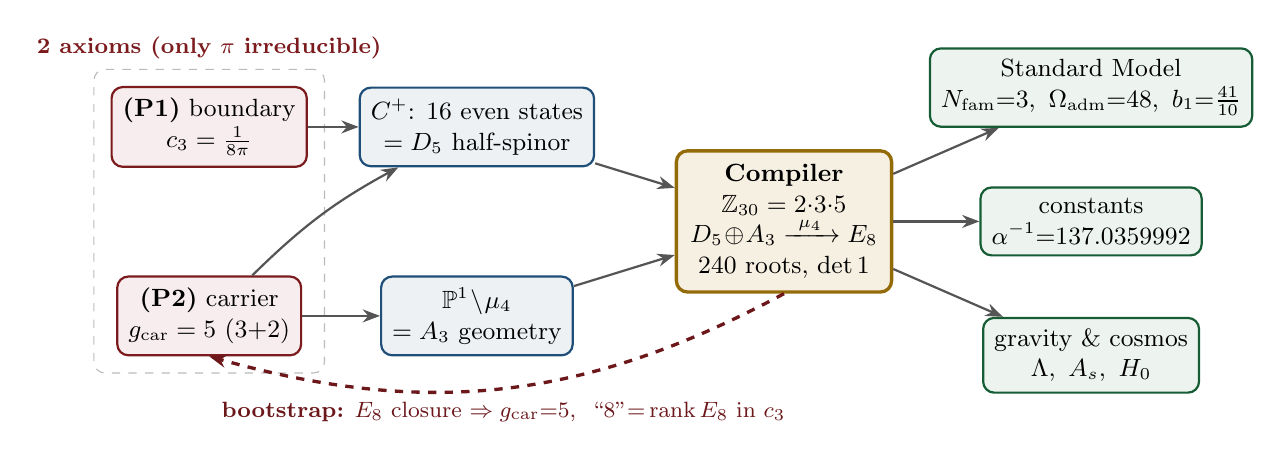
\begin{tikzpicture}[font=\small,
  inp/.style={rectangle,rounded corners,draw=tfred!80!black,fill=tfred!8,thick,align=center,inner sep=4pt,minimum height=10mm},
  atom/.style={rectangle,rounded corners,draw=tfblue,fill=tfblue!8,thick,align=center,inner sep=4pt},
  comp/.style={rectangle,rounded corners,draw=tfgold!80!black,fill=tfgold!12,very thick,align=center,inner sep=5pt},
  outp/.style={rectangle,rounded corners,draw=tfgreen!75!black,fill=tfgreen!8,thick,align=center,inner sep=4pt},
  ar/.style={-{Stealth[length=2.2mm]},thick,tfgray},
  back/.style={-{Stealth[length=2.2mm]},very thick,dashed,tfred!70!black}]
% inputs
\node[inp] (p1) at (0,1.2) {\textbf{(P1)} boundary\\$\cthree=\tfrac1{8\pi}$};
\node[inp] (p2) at (0,-1.2) {\textbf{(P2)} carrier\\$\gcar=5\ (3{+}2)$};
% atoms
\node[atom] (cp) at (3.4,1.2) {$C^+$: $16$ even states\\$=D_5$ half-spinor};
\node[atom] (a3) at (3.4,-1.2) {$\PP^1\!\setminus\!\mu_4$\\$=A_3$ geometry};
% compiler
\node[comp] (e8) at (7.3,0) {\textbf{Compiler}\\$\Z_{30}=2{\cdot}3{\cdot}5$\\$D_5\!\oplus\!A_3\xrightarrow{\ \mu_4\ }E_8$\\$240$ roots, $\det 1$};
% outputs
\node[outp] (sm)  at (11.2,1.7)  {Standard Model\\$\Nfam{=}3,\ \Oadm{=}48,\ b_1{=}\tfrac{41}{10}$};
\node[outp] (con) at (11.2,0.0)  {constants\\$\ainv{=}137.0359992$};
\node[outp] (cos) at (11.2,-1.7) {gravity \& cosmos\\$\Lambda,\ A_s,\ H_0$};
\draw[ar] (p1)--(cp); \draw[ar] (p2)--(a3);
\draw[ar] (p2) to[bend left=8] (cp);
\draw[ar] (cp)--(e8); \draw[ar] (a3)--(e8);
\draw[ar] (e8)--(sm); \draw[ar] (e8)--(con); \draw[ar] (e8)--(cos);
% --- BACK-CHANNEL: the bootstrap loop (E8 closure fixes the inputs) ---
\draw[back] (e8.south) to[bend left=22]
  node[below,font=\footnotesize,align=center,yshift=-1pt]{\textcolor{tfred!70!black}{\textbf{bootstrap:} $E_8$ closure $\Rightarrow \gcar{=}5$,\ \ ``$8$''${=}\operatorname{rank}E_8$ in $\cthree$}}
  (p2.south);
\begin{scope}[on background layer]
  \node[draw=tfgray!40,dashed,rounded corners,fit=(p1)(p2),inner sep=6pt,label=above:{\footnotesize\textcolor{tfred!80!black}{\textbf{2 axioms (only $\pi$ irreducible)}}}] {};
\end{scope}
\end{tikzpicture}
\end{center}

\noindent\textbf{Key statement (the loop closes):} previously $D_5$, $A_3$ and $E_8$ sat \emph{as given} Lie
structures in the background. Now they are \emph{intermediate products} of the two inputs --- \emph{and
the red back-channel is the new part}: the $E_8$ closure feeds back and \emph{fixes the inputs}.
$\gcar=5$ is the unique rank-fill/Coxeter/Pascal solution ($2^{g-1}=\binom g0{+}\binom g1{+}\binom g2$), and
the integer $8$ in $\cthree=\tfrac1{8\pi}$ is $\operatorname{rank}E_8=h(D_5)=\det R$. \textbf{Inputs and
output are mutually locked --- they prove each other}; the only thing \emph{not} produced by the loop is
the continuous $\pi$ (Möbius/Gauss--Bonnet), the lone irreducible primitive. So it is not a one-way arrow
chain but a closed self-consistency loop.

\medskip
\noindent\textbf{The master story is two engines.} Read from the two axioms, the whole theory factorises
into exactly \emph{two} engines --- a \emph{discrete} closure and a \emph{boundary} dressing. Gravity is
not a third block; it is the geometry channel of Engine~2.

\begin{center}
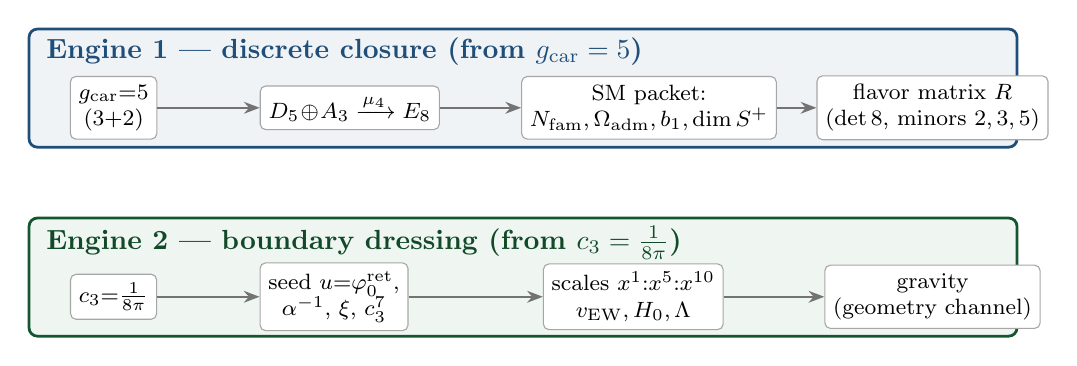
\begin{tikzpicture}[font=\small,
  eng/.style={rectangle,rounded corners=3pt,line width=1pt,inner sep=6pt,align=center},
  stp/.style={rectangle,rounded corners=2pt,draw=black!35,fill=white,inner sep=3pt,align=center,font=\footnotesize},
  ar/.style={-{Stealth[length=2mm]},thick,black!55}]
% Engine 1
\node[eng,draw=tfblue,fill=tfblue!7,text width=\linewidth,minimum height=15mm] (e1box) at (0,0) {};
\node[anchor=north west,font=\bfseries,tfblue] at (e1box.north west) {\;Engine 1 --- discrete closure (from $\gcar=5$)};
\node[stp] (a) at (-5.2,-0.25) {$\gcar{=}5$\\$(3{+}2)$};
\node[stp] (b) at (-2.2,-0.25) {$D_5\!\oplus\!A_3\xrightarrow{\mu_4}E_8$};
\node[stp] (c) at (1.6,-0.25) {SM packet:\\$\Nfam,\Oadm,b_1,\dim S^+$};
\node[stp] (d) at (5.2,-0.25) {flavor matrix $R$\\($\det 8$, minors $2,3,5$)};
\draw[ar] (a)--(b); \draw[ar] (b)--(c); \draw[ar] (c)--(d);
% Engine 2
\node[eng,draw=tfgreen!70!black,fill=tfgreen!7,text width=\linewidth,minimum height=15mm] (e2box) at (0,-2.4) {};
\node[anchor=north west,font=\bfseries,tfgreen!60!black] at (e2box.north west) {\;Engine 2 --- boundary dressing (from $\cthree=\tfrac1{8\pi}$)};
\node[stp] (f) at (-5.2,-2.65) {$\cthree{=}\tfrac1{8\pi}$};
\node[stp] (g) at (-2.4,-2.65) {seed $u{=}\phiz$,\\$\ainv$, $\xi$, $\cthree^7$};
\node[stp] (h) at (1.4,-2.65) {scales $x^1{:}x^5{:}x^{10}$\\$v_{\rm EW},H_0,\Lambda$};
\node[stp] (i) at (5.2,-2.65) {gravity\\(geometry channel)};
\draw[ar] (f)--(g); \draw[ar] (g)--(h); \draw[ar] (h)--(i);
\end{tikzpicture}
\end{center}

% =====================================================================
\section{The dependency DAG and the proof ledger}
% =====================================================================
The whole theory is a directed acyclic graph: two axioms at the source, the compiler in the middle, the
observables as sinks. The DAG makes the attack surface explicit --- each arrow is a named theorem or a
declared input, and each node fails in exactly one way.

\begin{center}
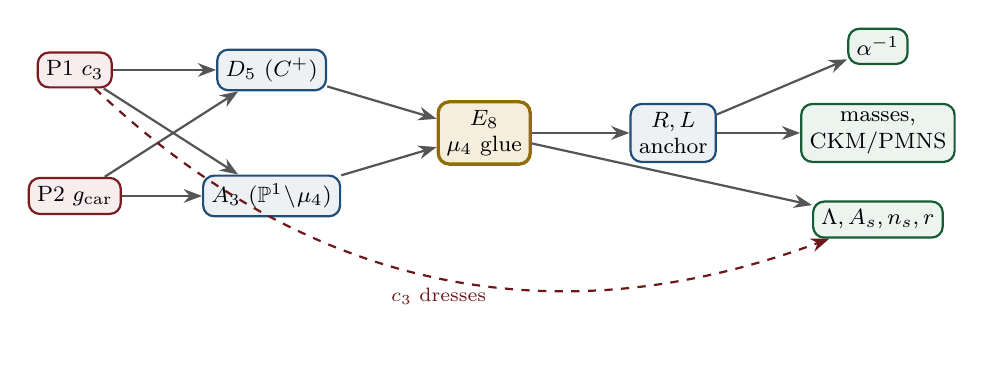
\begin{tikzpicture}[font=\footnotesize,>=Stealth,
  ax/.style={rectangle,rounded corners,draw=tfred!80!black,fill=tfred!8,thick,align=center,inner sep=3pt},
  nd/.style={rectangle,rounded corners,draw=tfblue,fill=tfblue!8,thick,align=center,inner sep=3pt},
  cp/.style={rectangle,rounded corners,draw=tfgold!80!black,fill=tfgold!14,very thick,align=center,inner sep=3pt},
  ou/.style={rectangle,rounded corners,draw=tfgreen!75!black,fill=tfgreen!8,thick,align=center,inner sep=3pt},
  ar/.style={->,thick,tfgray}]
  \node[ax] (p1) at (0,0.8) {P1 $\cthree$};
  \node[ax] (p2) at (0,-0.8) {P2 $\gcar$};
  \node[nd] (d5) at (2.5,0.8) {$D_5$ ($C^+$)};
  \node[nd] (a3) at (2.5,-0.8) {$A_3$ ($\PP^1\!\setminus\!\mu_4$)};
  \node[cp] (e8) at (5.2,0) {$E_8$\\$\mu_4$ glue};
  \node[nd] (rl) at (7.6,0) {$R,L$\\anchor};
  \node[ou] (al) at (10.2,1.1) {$\ainv$};
  \node[ou] (ms) at (10.2,0)   {masses,\\CKM/PMNS};
  \node[ou] (co) at (10.2,-1.1){$\Lambda,A_s,n_s,r$};
  \draw[ar](p1)--(d5); \draw[ar](p2)--(d5); \draw[ar](p1)--(a3); \draw[ar](p2)--(a3);
  \draw[ar](d5)--(e8); \draw[ar](a3)--(e8); \draw[ar](e8)--(rl);
  \draw[ar](rl)--(al); \draw[ar](rl)--(ms); \draw[ar](e8)--(co);
  \draw[ar,tfred!70!black,dashed] (p1) to[bend right=32] node[below,font=\scriptsize]{$\cthree$ dresses} (co);
\end{tikzpicture}
\end{center}

\begin{center}\scriptsize
\renewcommand{\arraystretch}{1.25}
\begin{tabularx}{\linewidth}{@{}p{1.5cm}p{3.0cm}p{1.5cm}cp{2.4cm}Y@{}}
\toprule
\textbf{Node} & \textbf{Definition} & \textbf{Inputs} & \textbf{St.} & \textbf{Output} & \textbf{Failure mode} \\
\midrule
P1 & RP boundary kernel, $\cthree{=}1/(8\pi)$ & --- (axiom) & \tA & $\cthree$ & no reflection-positive seam \\
P2 & $5$-slot carrier $\gcar{=}5$ & --- (axiom) & \tA & carrier $3{+}2$ & wrong family/charge lattice \\
$D_5$ & $C^+$ even-Hamming $=$ half-spinor $16$ & P2 & \tI & $\dim S^+{=}16$, $Y$ & group/matter mismatch \\
$A_3$ & $\PP^1\!\setminus\!\mu_4$ four-puncture geom. & P1 & \tI & $\Nfam{=}3$, $\Z_6$ & wrong multiplicity \\
$E_8$ & $\mu_4$ glue: $\operatorname{disc}{=}\Z_4$, $q$-sum$=2$ & $D_5,A_3$ & \tI & $240,248$ & not even-unimodular \\
$R,L$ & residue $+$ winding matrix, anchor $(1,1,2)$ & $A_3$ & \tI & $\det8$, minors $(2,3,5)$ & wrong $D_6$ branch \\
$\ainv$ & root of $F_{U(1)}(\alpha){=}0$ & $\cthree$, $M{=}41$ & \tN & $137.0359992$ & no/second root (excl.) \\
masses & $\phiz$-ladder $\lambda_Y^{L}\Lambda$ & $R,L$, $\cthree$ & \tI/\tP & $9$ masses, mixings & hierarchy mismatch \\
$\theta_{12}$ & TBM $+$ seam $\varepsilon{=}\cthree$ & $R,L$ & \tN/\tP & $0.307$ & seam-misalign.\ lemma fails \\
$\Lambda,A_s$ & seam det.\ / $R^2$ scalaron & $\cthree$ & \tP & $\Lambda$, $A_s,n_s,r$ & ambient RP fails \\
\bottomrule
\end{tabularx}
\end{center}

\markerkey
\noindent Reading the table top-to-bottom is reading the
theory: two red axioms in, everything else a consequence with exactly one failure mode each.

\begin{figure}[ht]
\centering
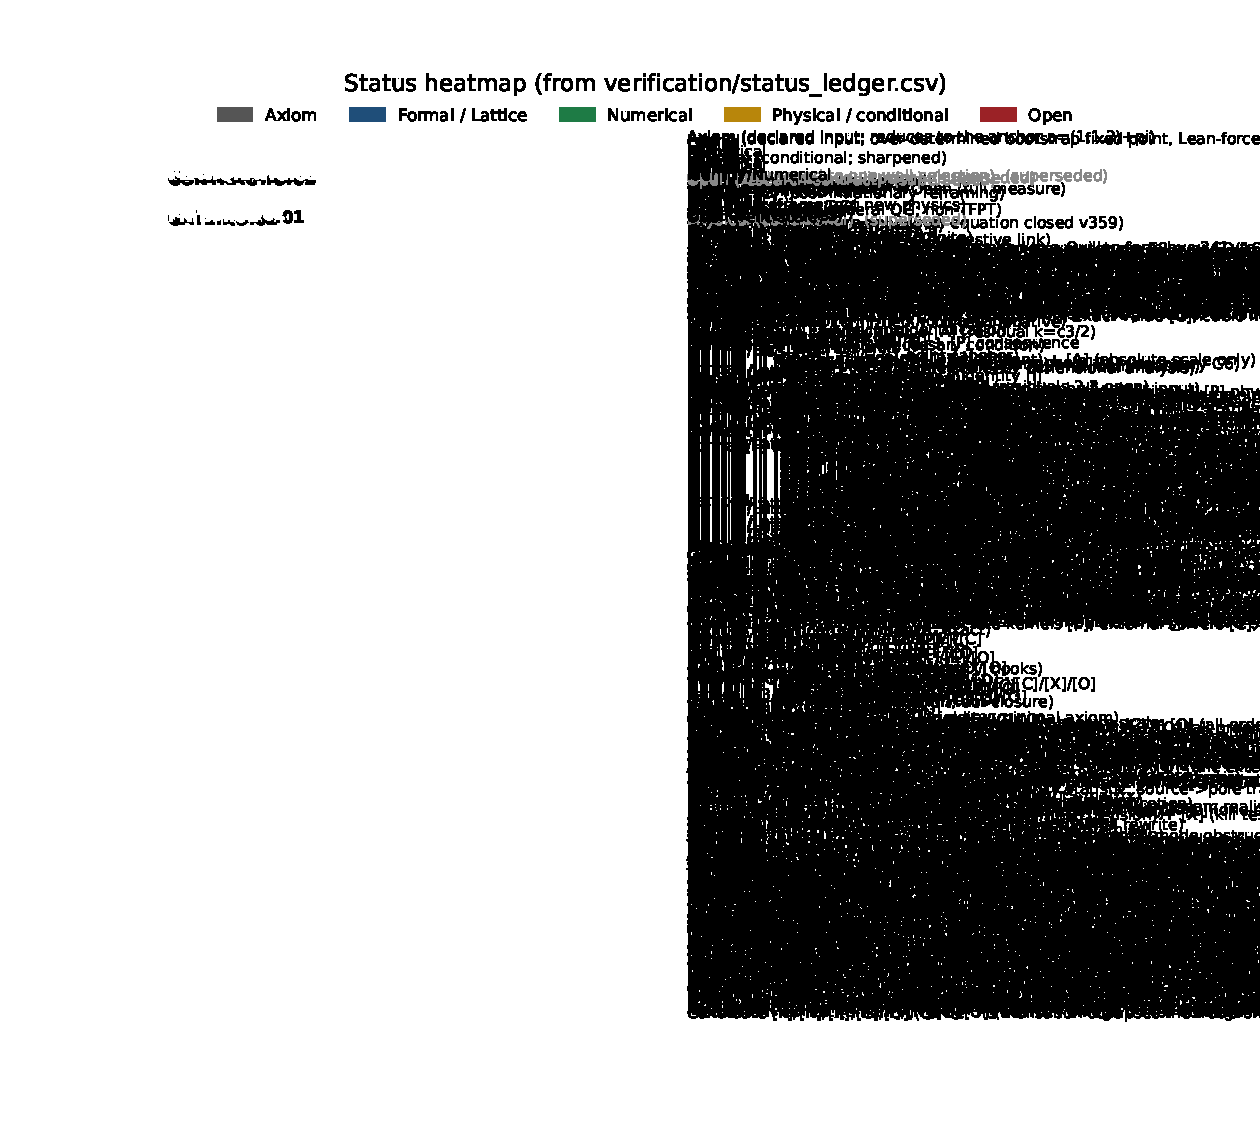
\includegraphics[width=0.92\linewidth]{figures/status_heatmap.pdf}
\caption{Status heatmap, generated directly from the single source of truth
\texttt{verification/status\_ledger.csv}. Grey $=$ axiom, blue $=$ formal/lattice, green $=$ numerical,
gold $=$ physical/conditional, red $=$ open. Each row carries a claim ID (\texttt{E8.GLU.01}, \dots) that
resolves to a ledger row with its dependencies and verification script. The ledger is \emph{versioned}: each
row has \texttt{active} and \texttt{canonical\_status}/\texttt{supersedes} fields, so claims that were later
superseded (e.g.\ the early ``flavor gate open'' rows, now \emph{ratios closed} via \texttt{FLAV.RIGID}) are
marked inactive and drawn dimmed --- the canonical status is the only one read as current.}
\label{fig:statusheat}
\end{figure}

\begin{keybox}[The compact status formula (three honest layers)]
\[
  \boxed{\ \underbrace{\text{compiler}}_{\text{closed}}\ \Big|\ 
  \underbrace{\text{admissible IR physics}}_{\text{conditionally closed (RP, gap)}}\ \Big|\ 
  \underbrace{\text{strict physical TOE}}_{\text{open}}\ }
\]
TFPT~5.0 closes the discrete compiler, the algebraic Standard-Model readout, the EM fixed point, the
admissible gapped IR sector and the $R+R^2$ spectral-action shadow. It does \emph{not} yet certify a strict
physical TOE. The remaining items have now collapsed sharply: the $R$-bridge amplitude normalisation
$U_{\mathrm{point}}$ \emph{reduces to} $v_{\mathrm{geo}}$ (Gate 1 closed, v75 --- the same anchor as $1/G$), and
the ambient metric measure is \emph{holographically reduced} to a finite seam-\emph{boundary} measure (Gate 2
tier B, v76) --- which is in turn the rigorously-constructed $(E_8)_1$ lattice net (v77), so $G_{\mathrm{metric}}$
is imported into existing RCFT rigor rather than built anew. So the only genuine residuals are \emph{one}
dimensionful scale $v_{\mathrm{geo}}$ --- the \emph{dimensional-analysis floor} that no theory escapes (v78),
shared by flavor and gravity --- the boundary net identification, and the named QFT/cosmology transfer
interfaces ($F_{\mathrm{frontier}}$).
\smallskip\\
\noindent\textbf{Two points that are \emph{not} in the residual (closed, but easy to mis-list as open).}
\emph{(i) Parameter-freeness is a theorem under the named hypotheses:} the boundary transport is gapped
($\Delta=6\log\tfrac32>0$), so by Perron--Frobenius its iteration has a \emph{unique} attracting fixed point
--- the constants are \emph{selected}, not tuned (\tI/\tL\ for the attractor, \veri{v56\_unique\_attractor.py};
the \emph{physical identification} of the transport operator stays \tP), reinforcing the
static bootstrap web ($\gcar=5$ forced three ways \emph{given} the $E_8$ closure rank --- a consistency
loop, see red team Target~B --- \veri{v6\_bootstrap.py}, \veri{v14\_carrier\_uniqueness.py}).
\emph{(ii) Newton's constant is not an \emph{independent} input:} fixing the physical $\Lambda$ branch
($(8\pi)^2\delta_{\mathrm{top}}=\tfrac{3}{4\pi^2}$) pins $\bar M_{\mathrm{Pl}}$ \emph{relative to} $\Lambda$, so
$G_N$ is read out \emph{after} the branch choice $+$ \emph{one} dimensionful induced-gravity anchor (\tI/\tP,
\veri{v60\_lambda\_metrology\_branch.py}), not predicted from pure numbers. What stays irreducible is then
just $\pi$, the discrete $E_8$-closure fixed point (self-consistent, \emph{not} a free axiom; the bootstrap of
\texttt{tfpt\_3}), and \emph{one} dimensionful scale $v_{\mathrm{geo}}$ --- and that single scale is shared by
\emph{both} the flavor sector ($U_{\mathrm{point}}\to v_{\mathrm{geo}}$, v75) and gravity ($1/G$, v68): the two
$[A]$ anchors are \emph{one} (dimensional analysis; no metre from pure mathematics).
\end{keybox}

\begin{keybox}[The hard reduction: everything open is two research gates plus typed interfaces]
After the compiler closure, the entire residual is
\[
  \boxed{\ \text{Rest}=(U_{\mathrm{wall}})\ \oplus\ (G_{\mathrm{metric}})\ \oplus\ (F_{\mathrm{frontier}})\ }
\]
--- one parabolic wall-selection, one quantum-gravity measure, and a set of deliberately typed
QFT/cosmology interfaces. \emph{Sharper aliases} (current state of the reductions; the historical gate
names are kept for ledger continuity): $(U_{\mathrm{wall}})\to v_{\mathrm{geo}}$ --- the flavor ratios are
\emph{closed} (Pl\"ucker/Readout Rigidity, v49/v71/v75), what remains is \emph{one dimensionful unit}, not a
flavor gap; $(G_{\mathrm{metric}})\to G_{\mathrm{net}}$ --- reduced to a single boundary-net theorem,
\emph{``the seam--Calder\'on net is the index-$4$ $\mu_4$ simple-current extension of the carrier net''}
(holomorphy then follows, v89/\texttt{GATE.METRIC.06}); $(F_{\mathrm{frontier}})\to F_{\mathrm{transfer}}$
--- named QFT/cosmology \emph{transfer} interfaces (Koide source$\to$pole, $\eta_B$ Boltzmann, axion relic,
$m_p/m_e$), never compiler powers. The status card:
\begin{center}\footnotesize
\renewcommand{\arraystretch}{1.18}
\begin{tabularx}{\linewidth}{@{}lcY@{}}
\toprule
\textbf{Item} & \textbf{Status} & \textbf{Reading} \\
\midrule
parameter-freeness (self-consistency) & \tI/\tL & gapped transport $\Rightarrow$ \emph{unique} Perron--Frobenius attractor (v56); bootstrap web $\gcar{=}5$ forced (v6/v14) \\
Newton constant $G_N$ & \tI/\tP & not \emph{independent}: branch pins $\bar M_{\mathrm{Pl}}$ rel.\ to $\Lambda$ (v60); readout after branch $+$ one dim.\ anchor \\
ratio $c_u/c_d=\tfrac{55}{117}$ & \tI & $\gcar\|\mathrm{Pl}_{\mathbf1,a}(K)\|_1/(\Nfam^2\Delta_Q)$; rigid on the derived stratum (v49/v71), no solve \\
$(U)$ flavor gate & \tA$\to v_{\mathrm{geo}}$ & \textbf{Gate 1 closed}: $U_{\mathrm{point}}{\to}v_{\mathrm{geo}}$ (ratios $+$ Grand Mass Volume, v75); same anchor as $1/G$ \\
$R+R^2$ gravity & \tI/\tP & covariant $f(R)$ field equation closed in regime; heat-kernel grounded (G2) \\
physical QG sector & \tF/\tP & gap-decoupled admissible measure ($\Delta_{\mathrm{eff}}{=}1.648{>}0$) \\
ambient QG measure & \tA (reduced) & \textbf{Gate 2 tier B}: holographically reduced to a finite seam-\emph{boundary} measure (v76); IR tier closed (decoupling); strict-TOE cert.\ open ($G_{\mathrm{metric}}$) \\
Koide & \tP & $Q_{\mathrm{src}}+\varphi_0/24$ as source$\to$pole transfer conjecture \\
axion DM & \tP/\tA & $f_a=M_{\mathrm{scal}}/128$ as a scenario \\
$\eta_B$ & \tP & readout closed; leptogenesis Boltzmann solve missing \\
$m_p/m_e$ & \tA & cross-sector QCD/EW ratio \\
$N_\star$ & \tP & reheating input, $N_\star\simeq57$ (continuous) \\
$a=(1,1,2)$ & \tL/\tP & forced by $4=2+1+1$, conditional on the carrier \\
$E_8$ Lean & \tF$\to$\tL & hardening, not a blocker (script-certified) \\
\bottomrule
\end{tabularx}
\end{center}
\markerkey
\noindent Only \emph{two} research gates remain --- $(U_{\mathrm{wall}})$ and $G_{\mathrm{metric}}$;
the frontier items are typed interfaces, not structural holes. Of these, $(U_{\mathrm{wall}})$ is the only
genuine \emph{physics} gate left: $G_{\mathrm{metric}}$ is now heat-kernel grounded (G2: the spectral action
gives $R+R^2$ structurally) and \emph{gap-decoupled} (G5: $\Delta_{\mathrm{eff}}{=}1.648{>}0$ isolates the
closed admissible sector from the un-built ambient), so its residual --- the ambient projective limit (G6)
--- is a \emph{strict-TOE completion target}: its absence does not affect the bounded IR claim, but it does
block certification as a strict physical TOE. Both are written up as numbered \emph{research contracts}
(lemma chains $+$ closing theorem $+$ machine-certifiability) in the companion
\texttt{tfpt\_research\_contracts}, with priority $(U_{\mathrm{wall}})$ first.
\veri{v36\_spectral\_action\_g2.py}
\end{keybox}

% =====================================================================
\section{Before / after: what concretely changes}
% =====================================================================
\begin{center}\small
\renewcommand{\arraystretch}{1.25}
\begin{tabularx}{\linewidth}{@{}p{3.5cm}YY@{}}
\toprule
\textbf{Aspect} & \textbf{State of Papers 1--7} & \textbf{After the compiler closure} \\
\midrule
$E_8$ & \emph{peripheral}: only an $11D{\to}4D$ reduction aside and the nilpotent-orbit \emph{cascade} (scale ordering) & \textbf{central, constructed}: $C^+{=}D_5$ spinor, $\PP^1\!\setminus\!\mu_4{=}A_3$, $\mu_4$ glue $\Rightarrow E_8$ \tL \\
$E_8$ numbers & $240,248$ read off tables when needed & $240{=}16{\cdot}5{\cdot}3$, $248{=}240{+}8$ \emph{derived} as carrier traces \tI \\
fine structure $\ainv$ & \emph{already} a parameter-free cubic fixed point $\alpha^3{-}2\cthree\alpha^2{-}8bc_6\ln(\cdot){=}0$, $\ainv{\approx}137.0365$ & \emph{same} equation, now \textbf{existence \& uniqueness proved} and refined to $137.0359992$; dev.\ $2.9\!\times\!10^{-10}$ vs CODATA-2022 ($1.9\sigma$) \tI/\tN \\
flavor residues & partly audit-flagged & anchor $\{1,1,2\}$ \& matrix forced by 3 hypotheses \tI/\tP \\
many sectors & side by side, each its own closure & \emph{one} compiler $\Z_{30}{=}2{\cdot}3{\cdot}5$ generates them \tI \\
inputs & $\cthree,\gcar$ (+ implicit structure) & exactly $2$ axioms (P1, P2), clearly declared \tA \\
$A_s$, $n_s$, $r$ (inflation) & scale present & scalaron mass fixed by $\cthree^7$ ($3.06{\times}10^{13}$ GeV); $A_s,n_s,r$ become \emph{predictions} \tP \\
$\theta_{12}$ (solar) & open (leading $\tfrac13$) & \textbf{cond.\ derived} $\tfrac13-\tfrac{\phiz}{2}=0.307$, given seam $\varepsilon{=}\cthree$ \tN/\tP \\
\bottomrule
\end{tabularx}
\end{center}
\markerkey

\begin{winbox}[Reduction in one line]
The number of \emph{structural} assumptions drops from ``a fixed-point seed $\cthree$, a carrier, the
orbit cascade, plus a per-sector calibration in each block'' to \textbf{two axioms}. Everything else
($\Nfam,\Oadm,b_1,\ainv$, the flavor matrix, the $E_8$ glue, the scale grammar) becomes a
\emph{consequence}. \emph{And even those two tighten:} the
bootstrap note shows $\gcar=5$ and the integer $8$ in $\cthree$ are \emph{overdetermined $E_8$-closure
fixed points} (rank-fill, Coxeter-match, integer-glue/norm all give $5$; $8=h(D_5)=\operatorname{rank}E_8=\det R=\varphi(30)$),
leaving \emph{one} genuine continuous primitive: $\pi$ from the Möbius boundary. So the \emph{discrete}
core has no freely tunable fundamental numbers --- the bootstrap is \emph{not creation from nothing} (two
inputs remain), but an overdetermination of those inputs. (This concerns the discrete core only;
dimensionful masses, the QG measure and frontier items remain typed-open.)
\end{winbox}

% =====================================================================
\section{Paper by paper: what each original paper did, and how it works now}
% =====================================================================
The seven original papers (plus the orientation note) total roughly \textbf{247 pages}. The table
below puts each one next to its compiler-era replacement: \emph{what} it treated and computed, \emph{how
many pages} it took, \emph{where} that now lives and how much it compresses, and whether the
\emph{accuracy} of the result improves on top. The honest summary up front: in most sectors the
\emph{numbers are the same} --- what shrinks dramatically is the \emph{derivation length} and the number
of independent assumptions; in three places (the solar angle, the inflation amplitude, the scalaron
mass) there is a \emph{genuinely new or sharper} result.

\begin{center}\footnotesize
\renewcommand{\arraystretch}{1.3}
\begin{tabularx}{\linewidth}{@{}p{0.7cm}p{3.5cm}cYc@{}}
\toprule
\textbf{P} & \textbf{Treated \& computed} & \textbf{Old} & \textbf{How it works now (note; compression)} & \textbf{Acc.} \\
\midrule
0 & orientation: architecture, decoder core $Y,[u_\Sigma],u$, theorem stack & 20\,p &
  \emph{one} compiler diagram: $\{\cthree,\gcar\}\!\to\!D_5{\oplus}A_3{\to}E_8$ (intro $+$ action\_grammar) & $=$ \\
1 & boundary kernel: $\cthree{=}\tfrac1{8\pi}$, Calder\'on polarization, carrier decoder $6Y^2{-}Y{-}\mathbf1{=}0$ & 20\,p &
  the two axioms P1 ($\cthree$) $+$ P2 ($\gcar{=}5$); carrier $=3{+}2$ atom (compiler) & $=$ \\
2 & carrier/SM packet: $S^+{=}16$, $G_{\mathrm{phys}}$, $\Nfam{=}3$, $\Oadm{=}48$, hypercharge, $b_1$ & 48\,p &
  compiler reads $16{=}1{+}5{+}10$, $\Nfam$, $\Oadm$, $b_1{=}\tfrac{41}{10}$ as carrier traces; $C^+{=}D_5$ spinor ($\sim$5\,p) & $=$ \\
3 & EM closure: $\ainv$ via $\sum L{+}N_\Phi{=}41$; flavor transport, CKM/PMNS, $\theta_{13}$ & 38\,p &
  $\ainv$ as unique root of $F_{U(1)}(\alpha){=}0$; flavor from transport theorem (parabolic $+$ sm) & $\uparrow$ \\
4 & admissibility/strong CP/QFT: $\theta_{\mathrm{eff}}{=}0$, OS reconstruction, mass gap & 40\,p &
  explicit gap $6\log\tfrac32$ $\Rightarrow$ Dobrushin/OS; strong CP from structure$+$RP (closing\_comp.) & $=$ \\
5 & geometric Hodge/metrology: $\Mpl$, $v_{\mathrm{geo}}$, $\Lambda$, spectral Einstein & 30\,p &
  Hodge/$R^2$ branch; $\Lambda$ \emph{typed} (one branch label); boundary-normalised (closing\_comp.) & $=$ \\
6 & cosmology interface: FRW, $\Lambda_{\mathrm{IR}}$, scalaron, reheating, leptogenesis, axion & 15\,p &
  Starobinsky $M{=}\cthree^{7/2}\Mbar{=}3.06{\times}10^{13}$ GeV; $A_s$ \emph{parameter-free} (closing\_comp.) & $\uparrow$new \\
7 & CMB operational closure: $C_\ell$, $a_{\ell m}$, seam mixer, Planck pipeline & 36\,p &
  $n_s{=}0.964$, $r{=}0.0040$ from the $R^2$ attractor, no free amplitude (closing\_comp.) & $\uparrow$new \\
\bottomrule
\end{tabularx}
\end{center}

\begin{winbox}[Three places where accuracy genuinely improves ``on top'']
\begin{enumerate}[leftmargin=1.6em]
\item \textbf{Solar angle $\theta_{12}$.} Paper 3 left it as the only open SM number (leading $\tfrac13$).
      It is now \emph{conditionally derived} (modulo the seam-misalignment lemma): TBM gives $\tfrac13$, the
      charged-lepton $1$--$2$ misalignment is the seam $\varepsilon=\tfrac{\Nfam}{|\mu_4|}\phiz=\tfrac34\phiz$
      (leading term exactly $\cthree{=}\tfrac1{8\pi}$), and TBM geometry gives
      $\sin^2\theta_{12}=\tfrac13-\tfrac23\varepsilon=\tfrac13-\tfrac{\phiz}{2}=0.3067$ --- $0.1\%$ from NuFIT.
\item \textbf{Inflation amplitude $A_s$.} Generic Starobinsky fits the scalaron mass to $A_s$. TFPT fixes
      it by the seam, $(M/\Mbar)^2=\cthree^7$, so $A_s=\tfrac{N_\star^2}{24\pi^2}\cthree^7=2.0\times10^{-9}$
      is a \emph{prediction} (Planck $2.1\times10^{-9}$), and the measured $A_s$ even \emph{predicts}
      $N_\star=56$.
\item \textbf{Scalaron mass.} $M=\cthree^{7/2}\Mbar=3.06\times10^{13}$ GeV comes out \emph{exactly} at the
      canonical Starobinsky value --- a number that was an input before is now an output.
\end{enumerate}
\end{winbox}

\noindent\textbf{What ``simpler'' means concretely.} The compression is not cosmetic. Paper 2 spent
$48$ pages establishing the carrier/SM packet by rigidity arguments; the compiler reads the same
$16{=}1{+}5{+}10$, $\Nfam{=}3$, $\Oadm{=}48$, $b_1{=}\tfrac{41}{10}$ off the Pascal row of a $5$-slot
carrier in a page. Paper 3's flavor transport ($38$\,p) becomes one transport theorem plus a fixed
residue matrix whose characteristic polynomial $t^3-9t^2+10t-8$ carries only compiler numbers. The
``many independent closures'' of Papers 1--7 become \emph{one} generator with a handful of corollaries.

% =====================================================================
\section{The compiler: why $30=2\cdot3\cdot5$}
% =====================================================================
The Coxeter number of $E_8$ is $h=30=2\cdot3\cdot5$. Exactly these three prime factors are the three
discrete atoms of the theory --- that is the point of the compiler:

\begin{center}
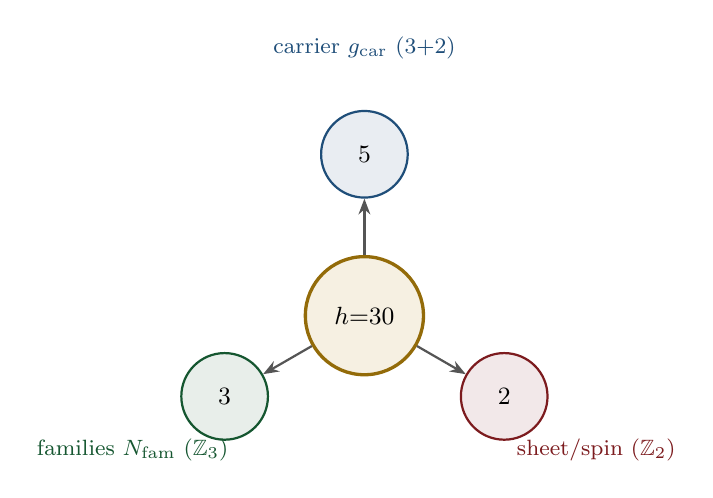
\begin{tikzpicture}[font=\small]
  \def\R{2.05}
  \node[circle,draw=tfgold!80!black,fill=tfgold!12,very thick,minimum size=15mm] (c) at (0,0) {$h{=}30$};
  \foreach \ang/\lab/\sub/\col in {90/$5$/{carrier $\gcar$ (3+2)}/tfblue, 210/$3$/{families $\Nfam$ ($\Z_3$)}/tfgreen!70!black, 330/$2$/{sheet/spin ($\Z_2$)}/tfred!80!black}{
    \node[circle,draw=\col,fill=\col!10,thick,minimum size=11mm] (n\lab) at (\ang:\R) {\lab};
    \draw[-{Stealth[length=2mm]},thick,tfgray] (c)--(n\lab);
    \node[\col,align=center,font=\footnotesize] at (\ang:{\R+1.35}) {\sub};
  }
\end{tikzpicture}
\end{center}

\noindent From this the compiler reads, among others:
\begin{itemize}[leftmargin=1.4em]
\item $\dim S^+ = 1+10+5 = 16$ (one generation) as the even exterior algebra of the $5$-slot carrier ---
      the same Pascal row $\binom50,\binom51,\binom52 = 1,5,10$ appears in family, action ladder and the
      $E_8$ root count. \tI
\item $|R(E_8)| = 16\cdot5\cdot3 = 240$ and $\dim E_8 = 240 + (5+3) = 248$. \tI
\item the $\Z_{30}$ Coxeter element $\leftrightarrow$ the cyclotomic polynomial $\Phi_{30}$; the corner
      rotation $z\mapsto iz$ on $\PP^1\!\setminus\!\mu_4$ is the $A_3$ Coxeter element. \tI
\end{itemize}

% =====================================================================
\section{The $\mu_4$ glue: how $E_8$ is really built}
% =====================================================================
The decisive, now \emph{proved} step: $D_5$ and $A_3$ have the \emph{same} discriminant group $\Z_4$, and
their discriminant-form norms are exactly two TFPT constants which add up to the $E_8$ root norm.

\begin{center}
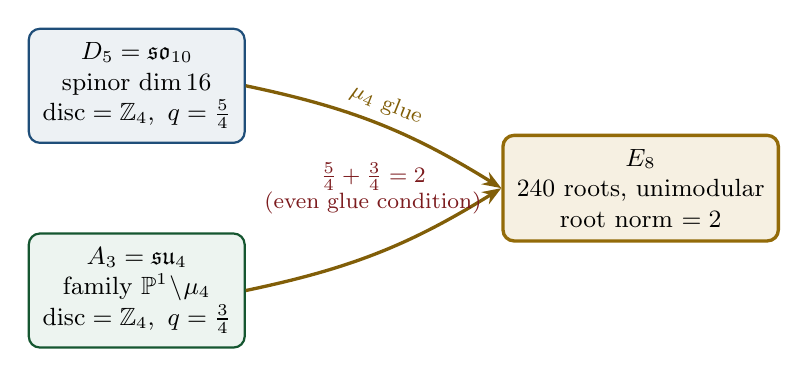
\begin{tikzpicture}[font=\small,
  bx/.style={rectangle,rounded corners,draw,thick,align=center,inner sep=5pt,minimum height=13mm}]
  \node[bx,draw=tfblue,fill=tfblue!8] (d5) at (0,0) {$D_5=\mathfrak{so}_{10}$\\spinor $\dim 16$\\$\operatorname{disc}=\Z_4,\ q=\tfrac54$};
  \node[bx,draw=tfgreen!70!black,fill=tfgreen!8] (a3) at (0,-2.6) {$A_3=\mathfrak{su}_4$\\family $\PP^1\!\setminus\!\mu_4$\\$\operatorname{disc}=\Z_4,\ q=\tfrac34$};
  \node[bx,draw=tfgold!80!black,fill=tfgold!12,very thick] (e8) at (6.4,-1.3) {$E_8$\\$240$ roots, unimodular\\root norm $=2$};
  \draw[-{Stealth[length=2.4mm]},very thick,tfgold!70!black] (d5.east) to[bend left=10] node[above,sloped,font=\footnotesize]{$\mu_4$ glue} (e8.west);
  \draw[-{Stealth[length=2.4mm]},very thick,tfgold!70!black] (a3.east) to[bend right=10] (e8.west);
  \node[align=center,font=\footnotesize,tfred!80!black] at (3.0,-1.3) {$\tfrac54+\tfrac34=2$\\(even glue condition)};
\end{tikzpicture}
\end{center}

\begin{keybox}[Glue theorem (proved)]
$\operatorname{disc}(D_5)=\operatorname{disc}(A_3)=\Z_4$, glue index $|{\mu_4}|=4$, and
$q(D_5)+q(A_3)=\tfrac54+\tfrac34=2=$ the $E_8$ root norm. Hence $E_8=(D_5\oplus A_3)+\mu_4$-glue is a
\emph{closed lattice-theoretic} construction --- not a blind ``positing of $248$''. \tL
\end{keybox}

% =====================================================================
\section{How derivation now works: the derivation map}
% =====================================================================
What can one concretely \emph{compute} with $\{\cthree,\gcar\}$? The following map summarises what is now
a consequence rather than an assumption.

\begin{center}\small
\renewcommand{\arraystretch}{1.2}
\begin{tabularx}{\linewidth}{@{}p{3.5cm}p{6.4cm}c@{}}
\toprule
\textbf{Sector} & \textbf{How it now arises} & \textbf{Status} \\
\midrule
gauge group / families & carrier $3{+}2$, $\dim S^+{=}16$, $\Nfam{=}3$, $\Oadm{=}48$ & \tI \\
hypercharge & roots of the charge polynomial $bsY^2+(s{-}b)Y-1$ & \tI \\
$U(1)$ index $b_1$ & $b_1=\dfrac{\gcar\,2^{\gcar-2}+1}{10}=\dfrac{41}{10}$ & \tI \\
fine structure $\ainv$ & unique root of $F_{U(1)}(\alpha)=0$ & \tI/\tN \\
flavor matrix & transport theorem (H1 proved, H2/H3 force the matrix) & \tI/\tP \\
electroweak scale & $v_{\mathrm{EW}}\sim e^{-\ainv/5}$ (carrier divides $\ainv$ by 5) & \tI \\
cosmological constant & $\Lambda\sim e^{-2\ainv}$ (density quotient; see typing note) & \tI/\tP \\
Hubble scale & $H_0\sim\sqrt{\Lambda}$ & \tP \\
inflation amplitude & $A_s=\dfrac{N_\star^2}{24\pi^2}c_3^7$ in the $R^2$ branch & \tP \\
$E_8$ & $D_5\oplus A_3+\mu_4$-glue & \tL \\
\bottomrule
\end{tabularx}
\end{center}
\markerkey

\noindent\textbf{Notable:} the scale grammar is \emph{one} exponential engine. The same number
$\ainv\approx137$ generates the electroweak scale (divided by $5=$ carrier), the cosmological constant
(times $2$) and --- via the square root --- the Hubble scale. One constant becomes many orders of
magnitude.

\smallskip
\noindent\textbf{Typing note on $\Lambda$ (a deliberate danger zone).} ``$\Lambda$'' denotes \emph{three}
distinct objects that must not be conflated: (i) the seam-determinant exponent $e^{-2\ainv}$ (an exact
\tI\ readout), (ii) the dimensionless density quotient $\rho_\Lambda/\Mbar^4$ (which carries a prefactor
\emph{branch}, hence \tP), and (iii) the observed curvature, to which (ii) is \emph{anchored}, not
predicted. The exponential is exact; the absolute dark-energy density remains a typed cosmology interface
(full disambiguation in \texttt{tfpt\_2\_standard\_model}).

\begin{keybox}[Cosmology is the Pascal action grammar of the carrier --- not a separate module]
With $x=v_{\mathrm{geo}}/(5\beta_{\mathrm{rad}}^2\Mbar)$ the cosmological readouts are a \emph{power tower}
on the five-slot carrier graph $K_5$:
\[
  \boxed{\ \frac{H_0}{\Mbar}=x^{5}R_H,\qquad \frac{\rho_\Lambda}{\Mbar^4}=x^{10}R_\Lambda\ },\qquad
  (1,5,10)=\tbinom50,\tbinom51,\tbinom52 .
\]
EW is the unit $x^1$, Hubble is the product over the $\binom51=5$ vertices, $\Lambda$ is the product over
the $\binom52=10$ edges --- the \emph{same} Pascal triple that reads one generation, the action ladder
and the $E_8$ root count $16\cdot5\cdot3=240$. ``Hubble $=$ slot product, $\Lambda=$ pair product.'' \tI
\end{keybox}

\begin{winbox}[The entire fermion spectrum in one formula]
Masses, Yukawa, CKM, PMNS and neutrinos all follow from \emph{one} master formula with \emph{one} seed:
\[
  \hat m_{f,j}=\frac{v_{\mathrm{geo}}}{\sqrt2}\,\lambda_Y^{\,L_{f,j}}\,\Lambda_{f,j},\qquad
  \lambda_Y=\sqrt{\phiz(1-\phiz)},\qquad \phiz=\tfrac1{6\pi}+\tfrac3{256\pi^4}.
\]
The word-lengths $L_{f,j}$ are the \emph{fixed residue matrix of the compiler}, whose characteristic
polynomial $t^3-9t^2+10t-8$ carries only compiler numbers ($\operatorname{tr}=9=\Nfam^2$,
$\det=8=h(D_5)$, principal $2$-minors $2{,}3{,}5$ with product $30=h(E_8)$). Through the $\phiz$-ladder
$\hat m=\tfrac{v_{\mathrm{geo}}\pi}{\sqrt2}c\,(\phiz)^k$ all nine word-lengths are fixed and the
\emph{charged-lepton} amplitudes are closed; the \emph{quark} mass \emph{ratios} are closed too (integer
Pl\"ucker readouts on the derived selector stratum, v49/v71), with only the \emph{absolute} amplitude scale
reducing to the $(U_{\mathrm{wall}})$ anchor.
\textbf{SM status:} the discrete packet, the dimensionless flavor skeleton, the charged-lepton source
masses and the quark \emph{ratios} are closed; the \emph{absolute} quark scale and the full PMNS completion
are reduced/conditional;
$m_W,m_Z,m_H,\sin^2\theta_W,\alpha_s$ are RG scheme-layer ($m_H$ rests on the closed UV quartic
$\tfrac1{16\pi^2}$); and the solar angle is \emph{realized by a TFPT texture} and reduced to the
seam-misalignment lemma ($\sin^2\theta_{12}=\tfrac13-\tfrac{\phiz}{2}$; see below). \emph{(Full derivation:
document~2, \texttt{tfpt\_2\_standard\_model}.)}
\end{winbox}

% =====================================================================
\section{Physical, geometric, topological: which solution is more plausible?}
% =====================================================================
\begin{center}\small
\renewcommand{\arraystretch}{1.22}
\begin{tabularx}{\linewidth}{@{}p{2.6cm}YY@{}}
\toprule
\textbf{Level} & \textbf{$E_8$ peripheral (v4.5)} & \textbf{$E_8$ compiled (new)} \\
\midrule
physical & $\ainv$ already a cubic fixed point, but each sector closed on its own & $\ainv$ as the fixed point of \emph{one} equation; one generator for many scales \\
geometric & Lie algebra external; $E_8$ only orders the cascade & the $C^+$ spinor $+$ puncture geometry $\PP^1\!\setminus\!\mu_4$ give $D_5,A_3$, glued to $E_8$ \\
topological & --- & the common discriminant $\Z_4$ ($\mu_4$ winding) forces the glue; $\Phi_{30}$/Coxeter drives the sectors \\
parsimony & many structures & $2$ axioms, the rest a consequence \\
\bottomrule
\end{tabularx}
\end{center}

\begin{winbox}[Why the compiled solution is more plausible]
It is (i) \emph{more parsimonious} (fewer independent assumptions $\Rightarrow$ less overfitting risk),
(ii) \emph{more rigid} (the glue condition $5/4+3/4=2$ and the discriminant $\Z_4$ leave little freedom),
and (iii) \emph{more checkable} (machine-checkable $E_8$ appendix, explicit fixed-point equation for
$\ainv$). More explained from less --- exactly the criterion that makes a theory more probable.
\end{winbox}

% =====================================================================
\section{What role $E_8$ now plays exactly}
% =====================================================================
$E_8$ is no longer the starting point but the \emph{output format}:
\begin{itemize}[leftmargin=1.4em]
\item \textbf{Bookkeeping:} $E_8$ is the unimodular container in which carrier ($D_5$) and family ($A_3$)
      fit together consistently. Its numbers $240,248$ are carrier traces, not inputs.
\item \textbf{Consistency test:} unimodularity ($\det 1$) is a hard condition; it closes only because the
      discriminant-form norms $5/4$ and $3/4$ (both already present in TFPT) add up to $2$. $E_8$ thus
      tests the internal coherence of the two atoms.
\item \textbf{Not an end in itself:} $E_8$ does not explain ``everything''; it is the smallest even
      unimodular hull of the datum $D_5\oplus A_3$. The physics sits in the \emph{two inputs}, not in
      $E_8$.
\end{itemize}

\noindent\textbf{New --- the secondary atlas.} Beyond that, $E_8$ is an \emph{audit container}: each
maximal subalgebra projects a TFPT module. Document~3 (\texttt{tfpt\_3\_e8\_audit\_bootstrap}, Part~I)
shows the seven slices of $248$ explicitly and labelled. The strongest new hit:
\begin{keybox}[$E_6\times A_2$ reads the flavor matrix]
\[
  248=\|R\|_F^2+\det R+2\,(\mathbf 1^\top R\,a)\,\Nfam=\underbrace{78}_{\dim E_6}+\underbrace{8}_{\dim A_2}+2\cdot27\cdot3 ,
\]
with $\|R\|_F^2=78=\dim E_6$, $\det R=8=\dim A_2=h(D_5)$. The discipline rule is: \emph{every load-bearing
number must appear in at least one $E_8$ projection} --- this makes the structure falsifiable rather than
numerological. (Audit level; all identities machine-verified.)
\end{keybox}

% =====================================================================
\section{What this means for the theory-of-everything question}
% =====================================================================
\needspace{0.46\textheight}
\begin{gapbox}[The state of the five questions --- closed, reduced or typed]
\begin{enumerate}[leftmargin=1.6em,itemsep=2pt,topsep=2pt]
\item \textbf{Flavor residual --- ratios closed; only the absolute scale is the wall-selection.}
      Mehta--Seshadri supplies the equivalence-class framework (stable parabolic $\leftrightarrow$ unitary
      representation); the algebraic selector $R$, the $Q$ spectrum and the splitting type are fixed (now
      \emph{derived}: $\det R=8$ lattice, $\operatorname{Spec}(Q_+)$ from $D_4$, v69/v70), and the
      charged-lepton amplitudes are closed. The quark mass \emph{ratios} ($c_u/c_d=\tfrac{55}{117}$ etc.) are
      then \emph{constant} on this discrete selector stratum (Readout Rigidity, v49/v71) --- integer Pl\"ucker
      readouts, no transcendental solve. Only the \emph{absolute} amplitude scale reduces to the selected
      \emph{polystable} point on the parabolic stability wall ($U_{\mathrm{point}}$, an anchor; Research
      Contract 1). \tI/\tA
\item \textbf{Gravity --- exact in the $R^2$ regime.} Spectral action $\to R{+}R^2$, BRST/Hodge kills the
      gauge directions, FRW reduction $\to$ Starobinsky; the only remainder is the \emph{controlled}
      low-curvature truncation ($R^{n\ge3}\!\to\!R^2$, valid for curvature $\ll M^2$). \tI\ in the regime
\item \textbf{Strong CP --- decoupled.} $\theta_{\mathrm{eff}}{=}0$ follows from three structural facts
      ($\gamma_5$-Hermiticity, polar structure, sheet involution) $+$ reflection positivity ---
      \emph{without} a mass gap. \tI\ (given RP)
\item \textbf{Full dynamics --- the admissible transfer model is closed.} The mass gap is the
      \emph{explicit} discrete gap $6\log\tfrac32$ of the $C_6$ transfer operator (eigenvalues $(k/3)^6$),
      which supports the OS reconstruction path on the admissible sector; the continuum and metric-coupled
      theory still require the stated RP, cluster and limit assumptions. \tI\ (transfer model) / \tP\ (continuum)
\item \textbf{Axioms P1/P2 --- P2 machine-verified.} The Lean proof builds cleanly (\texttt{1886 jobs},
      0 \texttt{sorry}, only kernel axioms); the P2 algebra is a theorem, P1 a typed interface. They
      remain declared inputs. \tI/\tA
\end{enumerate}
\end{gapbox}

\noindent In other words: the theory has shrunk from ``many open audit points'' to ``\emph{standard
steps} (cluster expansion, Fredholm, truncation bound) $+$ two declared axioms''. The five questions are
now \emph{closed, reduced or typed} rather than open-ended --- a qualitative jump in discipline, not a claim
of completion. \emph{(Details and proof chains: document~2, \texttt{tfpt\_2\_standard\_model}, Part~III.)}

\needspace{0.5\textheight}
\begin{keybox}[The TOE-completion ledger --- what is done, and what genuinely remains]
A theory-of-everything must close the discrete structure, the dimensionless constants, the mass
spectrum, gravity, and the quantum measure. The current state, graded honestly:
\begin{center}\footnotesize
\renewcommand{\arraystretch}{1.2}
\begin{tabularx}{\linewidth}{@{}p{4.6cm}cY@{}}
\toprule
\textbf{TOE piece} & \textbf{Status} & \textbf{If not complete: what closes it} \\
\midrule
gauge group, $\Nfam$, hypercharge, $b_1$ & \tI & --- complete \\
$E_8=(D_5{\oplus}A_3){+}\mu_4$, group closure & \tL & --- complete \\
bootstrap $(g,\mu){=}(5,4)$, ``$8$'' in $\cthree$ & \tL & --- complete (reverse glue $\mu^2{-}5\mu{+}4{=}0$) \\
fine structure $\ainv$ & \tN & --- \textbf{existence+uniqueness proved}; value is a numerical fixed point (ledger \texttt{EM.FP.01}), Ward origin \tP \\
fermion masses ($\phiz$-ladder) & \tI/\tA & leptons exact; quark \emph{ratios} closed (Pl\"ucker, v49/v71); absolute scale $=$ anchor \\
mixings $\theta_{13},\theta_{23},\theta_{12}$ & \tN/\tP & $\theta_{12}$ cond.\ derived; $\theta_{23}$ maximal \\
flavour matrix / H2 & \tI & up to Mehta--Seshadri unitarity (U), a Paper-3 input \\
inflation $A_s,n_s,r$, scalaron $M$ & \tN & parameter-free given $M_{\rm Star}{=}M_{\rm scal}$ \\
\midrule
\multicolumn{3}{@{}l}{\textit{genuinely open --- the actual TOE remainder}}\\
dim.\ EW/QCD masses & \tP & standard RG threshold matching (no new physics) \\
QFT measure (admissible sector) & \tI & \textbf{closed: RP from cusp spectrum, OS reconstruction} \\
ambient QFT $+$ full gravity (metric sector) & \tA & \emph{not constructed here} (frontier doc); conditionally reduces to one named hypothesis (ambient RP) on the relative spectral-action measure \\
analytic boundary origin of $\pi$ ($c_3{=}\tfrac1{8\pi}$) & \tP & \textbf{hardened: $c_3{=}1/(|\Z_2|\oint_{S^2}K)=1/(8\pi)$ (Gauss--Bonnet)}; ``$8$''${=}\operatorname{rank}E_8$; $\pi$ stays the one primitive \\
$\eta_B$, $m_p/m_e$, Koide, dark matter & \tA & frontier handles only (see document~4) \\
\bottomrule
\end{tabularx}
\end{center}
\end{keybox}
\markerkey

\noindent\textbf{The honest bottom line:} the discrete core, the dimensionless constants, the
\emph{mass-hierarchy exponents} and the mixings are \emph{closed}; the nine masses follow from one
$\phiz$-ladder (lepton rationals exact, quark $O(1)$ digits still a conditional finite evaluation). The
\emph{admissible-sector} QFT measure is closed (a finite gapped transfer system, RP from the cusp
spectrum, OS-reconstructed); the \emph{ambient/metric-sector} measure --- i.e.\ \emph{full quantum
gravity} --- is \emph{not} constructed here and stays \tA\ (frontier doc), reducing conditionally to a
single named hypothesis (ambient reflection positivity). The seam seed is \emph{hardened}:
$c_3=1/(|\Z_2|\oint_{S^2}K\,dA)=1/(8\pi)$ is the one-sided Gauss--Bonnet normalisation of the seam sphere,
with the discrete ``$8$'' equal to $\operatorname{rank}E_8$ and only the Gauss--Bonnet $\pi$ left as the
single irreducible primitive. What remains for a full TOE is then the ambient-RP hypothesis (full QG),
plus the standard-RG
dimensionful masses and the honest frontier items. No load-bearing discrete parameter remains free, and
$\pi$ is the lone continuous primitive.

% =====================================================================
\section{Does this make the theory more probable?}
% =====================================================================
\begin{keybox}[Plausibility balance]
\textbf{Pro:} (a) two inputs instead of many; (b) $\ainv$ to $2.9\times10^{-10}$ (CODATA-2022, $1.9\sigma$) as a \emph{fixed point},
not a fit; (c) $E_8$ constructed, not postulated; (d) one compiler generates several sectors $\Rightarrow$
fewer degrees of freedom, more predictive power.\\[2pt]
\textbf{Contra/open:} what remains are only \emph{standard steps} (cluster expansion in the thermodynamic
limit, the Fredholm property, the truncation bound) and the two declared axioms P1/P2; on the SM side the
dimensionful EW/QCD masses ($m_W,m_Z,m_H,\sin^2\theta_W,\alpha_s$) sit on the RG scheme layer. The solar
angle, previously the one open SM number, is now \emph{conditionally derived} ($\tfrac13-\tfrac{\phiz}{2}$,
modulo the seam-misalignment lemma). A final
verdict ``it maps reality'' requires this short list plus the near-term experimental tests (below).
\end{keybox}

Net: the parsimony (Kolmogorov-like compression: many numbers from little) and the high precision of
individual closures raise the a-posteriori plausibility substantially --- without hiding the open points.

% =====================================================================
\section{Predictions for running and upcoming experiments}
% =====================================================================
Because \emph{one} generator now sits behind the numbers, the theory makes a set of concrete, falsifiable
statements that running or near-term experiments are actively testing. Each row gives the TFPT value,
the \emph{new} derivation behind it, the experiment, and an honest status.

\begin{center}\footnotesize
\renewcommand{\arraystretch}{1.3}
\begin{tabularx}{\linewidth}{@{}p{2.5cm}p{4.9cm}Yc@{}}
\toprule
\textbf{Observable} & \textbf{TFPT value \& derivation} & \textbf{Experiment (running / upcoming)} & \textbf{St.} \\
\midrule
solar angle $\sin^2\theta_{12}$ &
  $\tfrac13-\tfrac{\phiz}{2}=0.3067$; TBM $+$ seam misalignment $\varepsilon=\tfrac34\phiz{\approx}\cthree$ (cond.) &
  \textbf{JUNO} (taking data since Aug 2025; sub-percent $\theta_{12}$) --- the sharpest live test & \tN/\tP \\
reactor angle $\sin^2\theta_{13}$ &
  $\phiz e^{-5/6}=0.0231$; seed $\times$ carrier-trace $e^{-\gamma}$, $\gamma{=}\tfrac56$ &
  Daya~Bay / RENO / JUNO (PDG $0.0220$) & \tI \\
atmospheric $\sin^2\theta_{23}$ &
  $\approx\tfrac12$ ($\mu\tau$-symmetric limit; octant not selected) &
  NOvA / T2K / \textbf{DUNE} (octant ambiguity, NuFIT~6.0) & \tP \\
fine structure $\ainv$ &
  $137.0359992$ as the unique root of $F_{U(1)}(\alpha){=}0$ (no fit, no second branch) &
  CODATA-2022 $137.035999177(21)$: dev.\ $2.9\times10^{-10}$ from the recommended adjustment ($1.9\sigma$ of its uncertainty) & \tI/\tN \\
tensor ratio $r$ &
  $r=\tfrac{12}{N_\star^2}=0.0040$ ($N_\star{=}55$); $R^2$ attractor, $M{=}\cthree^{7/2}\Mbar$ &
  now $r{<}0.036$ (BICEP/Keck BK18); \textbf{CMB-S4} ($\sigma_r\!\le\!5{\times}10^{-4}$, obs.\ $\sim$2033) & \tP \\
tilt $n_s$ &
  $n_s=1-\tfrac{2}{N_\star}=0.964$ (same attractor) &
  Planck ($0.965$); CMB-S4 sharpens & \tP \\
amplitude $A_s$ &
  $\tfrac{N_\star^2}{24\pi^2}\cthree^7=2.0\times10^{-9}$, parameter-free &
  Planck ($2.1\times10^{-9}$) & \tP \\
neutron EDM &
  $\theta_{\mathrm{eff}}=0\Rightarrow d_n$ essentially null (structure $+$ RP) &
  \textbf{PSI~nEDM} / SNS (running) & \tI \\
$0\nu\beta\beta$ / ordering &
  Majorana branch; normal-ordering preference &
  \textbf{LEGEND / nEXO}, DUNE, KATRIN & \tP \\
flavor invariants &
  $\det R{=}h(D_5){=}8$, principal minors $(2,3,5)$, $\chi_R{=}t^3{-}9t^2{+}10t{-}8$ (exact) &
  any future CKM/PMNS global fit must satisfy these & \tI \\
$H_0$ vs.\ $\Lambda$ &
  $v_{\mathrm{EW}}\sim e^{-\ainv/5}$, $\Lambda\sim e^{-2\ainv}$, $H_0\sim\sqrt\Lambda$: one engine &
  SH0ES / \textbf{DESI} / Planck (Hubble tension) & \tP \\
\bottomrule
\end{tabularx}
\end{center}
\markerkey

\begin{winbox}[The two decisive near-term tests]
\textbf{(1) JUNO and $\theta_{12}$.} JUNO is \emph{taking data since August 2025} and targets sub-percent
$\sin^2\theta_{12}$. TFPT commits to the conditional $\tfrac13-\tfrac{\phiz}{2}=0.3067$ (seam
$\varepsilon=\cthree$). A measured central value away from $\sim0.307$ at high significance falsifies the
seam mechanism --- a \emph{live} test.\\[2pt]
\textbf{(2) $r$.} The $R^2$ scalaron with $M$ fixed by $\cthree^7$ predicts $r=0.0040$ ($N_\star{=}55$),
already below the current bound $r<0.036$ (BICEP/Keck BK18) and within reach of CMB-S4
($\sigma_r\!\le\!5\times10^{-4}$, first observations $\sim$2033--34). A detection of $r\gtrsim0.01$ would be
incompatible with the $R^2$ branch on which $\Mpl$ and $A_s$ rest.
\end{winbox}

\noindent\textbf{Structural (non-experimental) checks.} Independent of any apparatus, the
machine-checkable $E_8$ appendix (all $240$ roots, Gram matrices, discriminant groups) lets anyone verify
that the two TFPT atoms really generate $E_8$; and the discipline rule ``\emph{every load-bearing number
appears in at least one $E_8$ projection}'' (atlas note) turns the number stock into a falsifiable raster
rather than numerology. The numerology charge itself is additionally \emph{quantified} by an explicit null
model: exhaustively enumerating a declared formula grammar (provably containing every scored TFPT formula)
against conservative data windows gives a joint look-elsewhere-corrected null probability $\le10^{-30.7}$
that a random theory of equal formula complexity reproduces the scorecard --- a statistical statement
conditional on the declared grammar, not a claim of certainty \tN\ \veri{v100\_numerology\_null\_mc.py}.

\begin{winbox}[Freeze file: committed kill criteria]
To prevent post-hoc rescue, the predictions above are frozen with explicit kill criteria in the
machine-readable registry \texttt{verification/freeze\_file.csv}. The decisive entries:
\begin{itemize}[leftmargin=1.4em,itemsep=1pt]
\item \textbf{solar} $\sin^2\theta_{12}=\tfrac13-\tfrac{\phiz}{2}\approx0.3067$ --- a JUNO central value clearly
  away from $0.307$ kills the seam-misalignment mechanism;
\item \textbf{tensor} $r\approx0.0040$ --- any robust $r\gtrsim0.01$ kills the $R^2$ branch carrying $\Mpl,A_s$;
\item \textbf{ordering} normal, small $m_{\beta\beta}$ --- inverted ordering or large $m_{\beta\beta}$ kills the
  Majorana branch;
\item \textbf{strong CP} $\theta_{\mathrm{eff}}=0$ --- a solid nEDM signal above SM background falsifies the
  structural cancellation;
\item \textbf{$w=-1$} --- a robust $w\neq-1$ kills the single-engine dark-energy readout.
\end{itemize}
The proton/electron ratio is explicitly \emph{not} claimed as a compiler power (only fails if mis-asserted as one).
\smallskip

\noindent\textbf{Blind-prediction registry (frozen 2026-06-09, machine-enforced).} Beyond the kill criteria,
the \emph{values} themselves are now frozen: \texttt{verification/predictions\_frozen.json} registers every
dimensionless prediction of record at $25$ significant digits \emph{before} JUNO / CMB-S4 / LiteBIRD / DESI
decide, and \veri{v84\_frozen\_registry.py} re-derives each decimal from the two axioms on every suite run
(formula$\leftrightarrow$value lock; covered by \texttt{manifest.sha256}; ledger \texttt{REG.FREEZE.01}).
In particular the registry admits exactly \emph{one} $\theta_{12}$ prediction of record (the seed
$\tfrac13-\tfrac{\phiz}2=0.306747$) --- the seam and non-linear variants are typed as derived variants of the
same texture and can never be silently promoted afterwards. $r$ and $n_s$ enter only as \emph{bands} over the
declared external $N_\star\in[50,60]$, never as point predictions.
\end{winbox}

\begin{winbox}[What likely follows next]
\begin{itemize}[leftmargin=1.4em]
\item the quark mass \emph{ratios} are now closed combinatorially (integer Pl\"ucker readouts on the derived
      selector stratum, v49/v69/v71); the only residual is the \emph{absolute} amplitude scale, an anchor
      ($U_{\mathrm{point}}$) of the same nature as the one dimensionful scale --- no new physics;
\item further constants as carrier traces (analogous to $b_1=41/10$), since the compiler systematically
      produces traces over $S^+$;
\item a sharper geometry$\leftrightarrow$gravity bridge once the Hodge/$R^2$ branch is lifted from
      \tP\ to \tI.
\end{itemize}
\end{winbox}

% =====================================================================
\section*{Conclusion}
% =====================================================================
\addcontentsline{toc}{section}{Conclusion}
The state of Papers 1--7 was an impressive collection of closures sharing common numbers. The compiler
closure explains \emph{why} they are the same numbers: a small discrete generator $\Z_{30}=2\cdot3\cdot5$
builds, from two inputs $\{\cthree,\gcar\}$ via $D_5\oplus A_3+\mu_4$, the $E_8$ container and outputs
the Standard Model, the constants and the scale grammar from there. The theory thereby becomes
\emph{more parsimonious, more rigid and more checkable}. Precisely nameable gaps remain --- one
geometric flavor realisation, the conditional gravity/QFT closures, and two declared axioms --- but the
path to closure is now short and concrete.

% =====================================================================
\section*{Appendix: computational verification (reproducibility)}
\addcontentsline{toc}{section}{Appendix: computational verification}
% =====================================================================
Every claim in this document marked \tI\ (exact identity), \tL\ (Lie/lattice theorem) or \tN\ (numerical
fixed point) is re-derived from the two axioms $\{\cthree,\gcar\}$ alone by a small, self-contained Python
suite in the repository folder \texttt{verification/}. The inline references \texttt{[verification/$\dots$]}
throughout the documents point to the exact script; the table below is the master map.

\begin{center}\small
\renewcommand{\arraystretch}{1.25}
\begin{tabularx}{\linewidth}{@{}p{3.5cm}Y@{}}
\toprule
\textbf{Script} & \textbf{What it machine-checks} \\
\midrule
\texttt{v1\_e8\_glue.py} & glue theorem $E_8{=}(D_5{\oplus}A_3){+}\mu_4$: $\operatorname{disc}{=}\Z_4$, $q(D_5){+}q(A_3){=}\tfrac54{+}\tfrac34{=}2$, $240{=}16{\cdot}5{\cdot}3$, $248{=}240{+}8$ \\
\texttt{v2\_carrier\_pascal.py} & $\gcar{=}5$ unique Pascal solution; $16{=}1{+}5{+}10$, $\Nfam{=}3$, $\operatorname{rank}E_8{=}8$, $\Oadm{=}48$, $b_1{=}\tfrac{41}{10}$ \\
\texttt{v3\_em\_alpha.py} & EM closure: unique root of $F_{U(1)}(\alpha){=}0$, $\ainv{=}137.0359992168$, existence/uniqueness, inverse test, ablation \\
\texttt{v4\_flavor\_matrix.py} & residue matrix $R$: $\det{=}8$, minors $\{2,3,5\}$, $\chi_R{=}t^3{-}9t^2{+}10t{-}8$, SNF $\operatorname{diag}(1,1,8)$, $\|R\|_F^2{=}78$, $\sum L{=}40$ \\
\texttt{v5\_e8\_cascade.py} & cascade $D_n{=}60{-}2n$: endpoints, exponent rungs $\to240$, IR tail $46080$, variance $6552$ \\
\texttt{v6\_bootstrap.py} & reverse glue $\mu^2{-}5\mu{+}4{=}0$; $\gcar{=}5$ three ways; $8{=}\operatorname{rank}E_8{=}h(D_5){=}\varphi(30)$ \\
\texttt{v7\_gravity\_cosmo.py} & scalaron exponent $7$, $M_{\rm scal}^2/\Mbar^2{=}\cthree^7$, $A_s,n_s,r$, $\Omega_b$, $\sin^2\theta_{12}$ \\
\texttt{v8\_horizon.py} & horizon code: $\tfrac1{2\pi}{=}4\cthree$, $1920{=}|W(D_5)|$, $S_{dS}$, Page, $\beta_{\rm rad}{=}0.2424^\circ$ \\
\texttt{v9\_neutrino\_texture.py} & solar angle: explicit $\mu\tau$ Majorana texture $\to\sin^2\theta_{12}{=}\tfrac13{-}\tfrac{\phiz}2$, $\theta_{23}{=}45^\circ$, $\theta_{13}{=}0$ \\
\texttt{v10\_\allowbreak projection\_\allowbreak involution.py} & $Q,\Sigma$ algebra: $K{=}R{+}Q\Sigma$, $L{=}R{+}Q(I{+}\Sigma)$; $\chi_Q,\chi_K$; det ladder $3{\cdot}4{\cdot}8{\cdot}20{=}1920{=}|W(D_5)|$; $a^\top Ka{=}41$ \\
\texttt{v11\_unique\_KQ.py} & $K,Q$ are the \emph{unique} nonneg-int matrices with their compiler budgets, spectrum and monotone rows (enumeration) \\
\texttt{v12\_\allowbreak mass\_\allowbreak generation\_\allowbreak polynomials.py} & sector/generation polynomials of $K$ and the anchor-block det ladder $(9,10,16,40)$ \\
\texttt{v13\_open\_gates.py} & gate closures: $M{=}41{=}10b_1{=}\sum L{+}N_\Phi$; $Q_+$ $=$ $A_3$ exponents, $Q_-^2{=}\Nfam$ \\
\texttt{v14\_\allowbreak carrier\_\allowbreak uniqueness.py} & $\gcar{=}5$ unique ($\Nfam\in\Z^+$, rank $E_8{=}8$); split $(3,2)$ from $b{+}s{=}5,b^2{+}s^2{=}13$; $\operatorname{Tr}Y{=}\operatorname{Tr}Y^3{=}0$ \\
\texttt{v15\_\allowbreak bootstrap\_\allowbreak classification.py} & $D_5{\oplus}A_3$ unique familyful cyclic-glue of $E_8$ ($16$-spinor $+$ $3$ families), glue $\Z_4$ \\
\texttt{v16\_\allowbreak solar\_\allowbreak dual\_\allowbreak anchor.py} & $a^\top R^{-1}{=}a^\top L^{-1}{=}(-\tfrac12,-\tfrac12,1)$; $\sin^2\theta_{12}{=}\tfrac13{-}\tfrac{\phiz}{2}$; full PMNS \\
\texttt{v17\_\allowbreak hexagonal\_\allowbreak resolvent.py} & finite resolvent $D_y^{-1}{=}(\sum y^{5-m}\delta^m U_6^m)/(y^6{-}\delta^6)$ (quark $c$ backbone) \\
\texttt{v18\_quark\_yukawa.py} & quark source ratios $\tfrac{m_u}{m_d}{=}0.470085,\tfrac{m_c}{m_s}{=}13.61,\tfrac{m_t}{m_b}{=}40.80$ exact; lepton $c{=}(\tfrac{16}{7},\tfrac43,\tfrac76)$; full hierarchy \\
\texttt{v19\_\allowbreak monodromy\_\allowbreak moduli.py} & exact pole $z_\star{=}\tfrac{794-7\sqrt{9961}}{2187}$ ($3^7$); $D_4$ $SU(3)$ monodromy constructible but $D_4$-fixed locus positive-dim $\Rightarrow$ exact quark $c$ reduce to $(U)$ \\
\texttt{v20\_\allowbreak lepton\_c\_\allowbreak derivation.py} & lepton $c$'s derived: $\delta{=}\tfrac12$ resolvent $c{=}|\mu_4|^w/(\tfrac54{-}\cos\tfrac{r\pi}3)$ $\Rightarrow$ $\tfrac{16}7,\tfrac43$; product $\tfrac{2^{\gcar}}{\Nfam^2}{=}\tfrac{32}9$ $\Rightarrow$ $\tfrac76$ \\
\texttt{v21\_\allowbreak solar\_\allowbreak product\_\allowbreak quark.py} & solar coeff $=q(A_3){=}\tfrac34$ (glue-norm, $q(D_5){+}q(A_3){=}2$), $\sin^2\theta_{12}{=}\tfrac13{-}\tfrac{\phiz}2$; product $\tfrac{2^{\gcar}}{\Nfam^2}$; quark law fails ($\tfrac17$ vs $0.724$) \\
\texttt{v22\_\allowbreak open\_gates\_\allowbreak audit.py} & residual-gates audit contract: exact reduction of each open gate (A2,B3,B4,B5,B6,C7) machine-pinned (forced part vs.\ named residual) \\
\texttt{v23\_\allowbreak anchor\_\allowbreak generator.py} & anchor $a{=}(1,1,2)$: $e_k{=}(4,5,2)$, $\cthree{=}\tfrac1{2e_1\pi}$; $p_n{=}2{+}2^n\!\Rightarrow\!240,248$, binary ladder; inputs $\to\{a,\pi\}$ \\
\texttt{v24\_\allowbreak quark\_\allowbreak ratio\_\allowbreak closure.py} & quark ratios $\tfrac{55}{117},\tfrac{34}{47},\tfrac3{26}$ from TFPT blocks; mass ratios match $<0.03\%$; rational $c$ gauge, $\Lambda_q$ in $O(1)$ \\
\texttt{v25\_\allowbreak frontier\_\allowbreak conjectures.py} & conjectures: Koide $Q_{\mathrm{src}}{+}\tfrac{\phiz}{24}{\approx}\tfrac23$; axion $f_a{=}M_{\mathrm{scal}}/128{\to}m_a{\approx}23.8\,\mu$eV \\
\texttt{v26\_\allowbreak flavor\_frontier\_\allowbreak unification.py} & the ``$11$'' is not uniquely forced ($\Rightarrow$\,\tP); flavor frontier unifies to one $(U)$ gate; cusp config on the parabolic stability wall \\
\texttt{v27\_\allowbreak wall\_\allowbreak representative.py} & explicit balanced wall rep $W_{\mathrm{wall}}$ (cols $=$ perm$(0,1,2)$, rows $w{=}(2,1,1)$, pardeg $0$); selector $\det R{=}8$, $\mathrm{Spec}(Q_+){=}\{1,2,3\}$ \\
\texttt{v28\_\allowbreak gravity\_\allowbreak fR.py} & $R{+}R^2$ closed: $f(R)$, $M{=}\cthree^{7/2}\Mbar$ scalaron, $N_\star{=}57\!\to\!n_s,r,A_s$; full metric measure open; $248\cthree^2{<}6\log\tfrac32$ \\
\texttt{v29\_\allowbreak research\_contract\_\allowbreak certs.py} & research-contract certificates: $C_U^{(1)}$ wall enumeration ($1296{\to}144{\to}5$ orbits; symmetry alone does not pick $W_{\mathrm{wall}}$) and $G5$ gap-dominance $2\|V\|{<}\Delta$ \\
\texttt{v30\_\allowbreak d4\_character\_\allowbreak variety.py} & $C_U^{(2)}$: full $D_4$-fixed $SU(3)$ character variety is positive-dimensional $\Rightarrow$ selector needs the $R(\rho)$ dictionary (H2) --- the single remaining $(U_{\mathrm{wall}})$ input \\
\texttt{v31\_\allowbreak R\_\allowbreak dictionary.py} & $R(\rho)$ characterized: case A alive (irreducible $\Rightarrow$ mixing); $R$ integer but $\rho$-invariants continuous $\Rightarrow$ $R(\rho)$ is the transcendental non-abelian-Hodge map (residual $=$ Hitchin solve) \\
\texttt{v32\_\allowbreak rh\_\allowbreak splitting.py} & RH route: $\sum_kU^kA_0U^{-k}{=}4\operatorname{diag}(A_0)$ exact $\Rightarrow$ splitting $\mathcal O(-2){\oplus}\mathcal O(-1)^2\!\Leftrightarrow\!\operatorname{diag}(A_0){=}(\tfrac12,\tfrac14,\tfrac14)$ (algebraic); $\prod M_k{=}I$ + $R$-bridge stay open ($c_u/c_d$ not forced) \\
\texttt{v33\_\allowbreak explicit\_flat\_\allowbreak bundle.py} & explicit valid $(U_{\mathrm{wall}})$ flat bundle (RH solve): cusp $+$ $\mathcal O(-2){\oplus}\mathcal O(-1)^2$ $+$ $\|M_\infty{-}I\|{\sim}10^{-9}$ ($\prod M_k{=}I$) $+$ irreducible (case A) \\
\texttt{v34\_\allowbreak h2\_bridge\_\allowbreak attempt.py} & H2 bridge: explicit per-puncture $M_k$ (cusp, $\prod M_k{=}I$); honest negative --- natural extraction $\neq$ lepton amplitudes, the $\Gamma^{\min}$ dictionary is the remaining input ($c_u/c_d$ not obtained) \\
\texttt{v35\_\allowbreak quark\_qcd\_\allowbreak boundary.py} & the open gates are the discrete$\leftrightarrow$continuous boundary: quark cross-ratio cleanness tracks generation/QCD sensitivity (compiler hands off to continuous physics) \\
\texttt{v36\_\allowbreak spectral\_action\_\allowbreak g2.py} & G2: spectral action $\to R{+}R^2$ ($a_2{\sim}{-}R/3$, $a_4|_{R^2}{\sim}R^2/72$); $M^2/\Mbar^2{=}6(4\pi)^2/f_0$, $\cthree^7$ fixes $f_0$; gap-decoupling $\Delta_{\mathrm{eff}}{=}1.648{>}0\Rightarrow$ admissible IR closed under RP, ambient (G6) $=$ strict-TOE completion target \\
\texttt{v37\_\allowbreak plucker\_\allowbreak anchor.py} & anchor-plane Plücker apparatus: $\|\mathrm{Pl}(K)\|_1{=}11$, $\|\mathrm{Pl}_R(K)\|_1{=}26$, $\sum\mathrm{Pl}_R(L){=}60$; pencil $\det(K{+}xQ){=}3x^3{+}7x^2{+}6x{+}4$; $K_e{-}K_u{=}a$, $L_e{-}L_u{=}\mathrm{Exp}(A_3)$; lepton ring $c_ec_\tau{=}|\Z_2|c_\mu$; Koide $u{\to}\tfrac{53}{54}u$ (\tP) \\
\texttt{v38\_\allowbreak uwall\_\allowbreak killswitch.py} & $(U_{\mathrm{wall}})$ U2 kill-switch hardened: $D_4$-cusp rep irreducible at all $400$ sampled points (commutant${=}1$), mixing ${\ge}0.35$, reducible locus measure-zero $\Rightarrow$ case A generic, $(U_{\mathrm{wall}})$ survives; amplitude dictionary still research-level \\
\texttt{v39\_\allowbreak uwall\_\allowbreak selectors.py} & $(U_{\mathrm{wall}})$ selector side closed on the explicit point: splitting type ${=}$ anchor $a{=}(1,1,2)$, pardeg ${=}0$; $\det R{=}8{=}n{\cdot}a$, $\mathrm{Spec}(Q_+){=}\{1,2,3\}{=}3\alpha{+}1$ read off the bundle; only the amplitudes $c_u/c_d$ ($\Gamma^{\min}$ Hitchin) remain \\
\texttt{v40\_\allowbreak harmonic\_\allowbreak metric.py} & $(U_{\mathrm{wall}})$ harmonic metric ${=}$ FINITE linear algebra (polystable${\Rightarrow}$unitary${\Rightarrow}\Phi{=}0$): unique invariant form $H{>}0$, unitarised $\widetilde M_k$ cusp-class with $|\widetilde M_k|{\in}\{0,\tfrac12,\tfrac1{\sqrt2}\}$; the feared Hitchin PDE collapses to unitarisation $+$ combinatorial $R$ \\
\texttt{v41\_\allowbreak leg\_\allowbreak assignment.py} & $(U_{\mathrm{wall}})$ final leg test: amplitudes ${=}$ $\delta{=}\tfrac12$ resolvent (closed); $\Lambda_\mu{>}1$ rules out holonomy moduli; harmonic holonomy $|\mathrm{diag}|{=}(0,\tfrac12,\tfrac12)$ supplies $\delta{=}\tfrac12$ (suggestive); honest negative on literal $c_u/c_d$ reproduction \\
\texttt{v42\_\allowbreak exterior\_\allowbreak leg.py} & $(U_{\mathrm{wall}})$ Exterior Leg Lemma: $u,d$ share $(r,w){=}(1,1)$ so any scalar leg gives $c_u/c_d{\equiv}1$; the $u/d$ split is the $\Lambda^2F$ area $\mathrm{Pl}_{\mathbf1,a}(K)$, $\|{\cdot}\|_1{=}11$ generated $\Rightarrow$ $\tfrac{5\cdot11}{9\cdot13}{=}\tfrac{55}{117}$ \tI; phys.\ identification \tP\ \\
\texttt{v43\_\allowbreak exterior\_\allowbreak bridge.py} & $(U_{\mathrm{wall}})$ $\Lambda^2F$ bridge: $\Lambda^2(\widetilde M){=}\overline{\widetilde M}$ (exterior leg ${=}\mathbf{\bar3}$) confirmed; continuous action $\neq$ integer $\mathrm{Pl}(K)$ $\Rightarrow$ bridge is the discrete H2 invariant ($\det R{=}8$, $\mathrm{Spec}(Q_+)$ confirmed), not continuous \\
\texttt{v44\_\allowbreak carrier\_\allowbreak exterior.py} & $(U_{\mathrm{wall}})$ Lie-level grounding: $16{=}\Lambda^{\mathrm{even}}(5){=}1{+}10{+}5$; $u^c{\in}\Lambda^2(5)$, $d^c{\in}\Lambda^4(5)$ $\Rightarrow$ exterior degrees $(2,4)$, sum${=}6{=}|R^+\!(A_3)|$, diff${=}2{=}|\Z_2|$; the exterior leg is the carrier's own $\Lambda^2$ grading (no special math) \\
\texttt{v45\_\allowbreak family\_\allowbreak exterior.py} & $(U_{\mathrm{wall}})$ the ``$11$'' is Pascal: $|\mathrm{Pl}(K)|{=}(1,4,6){=}\{\Lambda^0,\Lambda^1,\Lambda^2\}(\mu_4)$; $\|\mathrm{Pl}(K)\|_1{=}11{=}\sum_{k\le2}\binom4k{=}16{-}\gcar$ (cumulative ext of $\mu_4$ up to $\deg u^c{=}2$); $15{=}\dim\mathfrak{su}(4){=}10{+}5{=}\Nfam\gcar$ \\
\texttt{v46\_\allowbreak grand\_mass\_\allowbreak volume.py} & absolute mass-scaling is \tI, not a product rule: sector dets $(\phiz)^{6},(\phiz)^{9},(\phiz)^{10}$ (exponents $|R^+\!A_3|,\Nfam^2,\mathcal A_\Lambda$) $\Rightarrow$ $\det M_{\mathrm{SM}}{\sim}(\phiz)^{25}{=}(\phiz)^{\gcar^2}$; $Q$-rows $(4,5,6)$ sum $15{=}\dim A_3$; $25{+}15{=}40{=}\sum L$ \\
\texttt{v47\_\allowbreak selection\_\allowbreak theorem.py} & Boundary Carrier Selection (Thm A): $\mu_4{\to}A_3,\Nfam{=}3$; $16$-spinor${\to}D_5$; $q(D_5){+}q(A_3){=}2$, glue $4{=}|\mu_4|$; only $D_5{\oplus}A_3$ meets all four conditions ($D_8,E_7{+}A_1,E_6{+}A_2,A_4{+}A_4,A_8$ excluded) \tL/\tP \\
\texttt{v48\_\allowbreak em\_ward.py} & EM boundary Ward (Thm C): $F_{U(1)}{=}$ Maxwell $\alpha^3$ $-$ Calder\'on $2\cthree^3\alpha^2$ $-$ transport $8b_1\cthree^6\log\tfrac1{\varphi_{\mathrm{seam}}}$; $8b_1{=}\tfrac45 M{=}\tfrac{164}5$, $-\tfrac54{=}q(D_5)$ \tI; Ward origin \tP \\
\texttt{v49\_\allowbreak readout\_\allowbreak rigidity.py} & Readout Rigidity (Thm U2): $c_u/c_d{=}\tfrac{55}{117}$ is constant on the discrete selector stratum $\mathcal S_{8,Q}$ $\Rightarrow$ no point-uniqueness needed; $(U_{\mathrm{wall}}){=}U_{\mathrm{unitary}}{+}U_{\mathrm{H2}}{+}U_{\Lambda^2}{+}U_{\mathrm{point}}$, only $U_{\mathrm{point}}$ open \\
\texttt{v50\_\allowbreak q\_geometry.py} & Q geometry (Thm Q): $Q_+{=}$ diag$(3,2,1)$-block $\chi{=}(t{-}1)(t{-}2)(t{-}3)$, $Q_-$ $\chi{=}t(t^2{-}3)$; $Q$ unique under rows$(4,5,6)$/cols$(9,5,1)$/spectra; geom.\ origin \tP \\
\texttt{v51\_\allowbreak boundary\_\allowbreak half\_step.py} & glue norms ${=}(\gcar,\Nfam)/|\mu_4|$: $q(D_5){=}\tfrac54$, $q(A_3){=}\tfrac34$; four ops forced ${\to}$ $\{$sum$=2$ root norm, diff$=\tfrac12{=}|\Z_2|/|\mu_4|{=}\delta$, prod$=\tfrac{15}{16}$, ratio$=\tfrac53\}$. So $\delta{=}\tfrac12$ is the carrier$-$family count over the glue index, not chosen \tI \\
\texttt{v52\_\allowbreak pencil\_\allowbreak endpoints.py} & $K{+}xQ$ pencil endpoints: $P({-}1){=}2{=}|\Z_2|$, $P(0){=}4{=}|\mu_4|$, $P(1){=}20{=}\det L$, $P(2){=}68{=}2p_5(a)$; $\det(K{-}Q){=}2$, $\operatorname{tr}{=}\Nfam$ (audit ext.\ of v37) \tI \\
\texttt{v53\_\allowbreak compiler\_\allowbreak core.py} & Big picture: the whole integer skeleton from $(\gcar,\Nfam){=}(5,3)$ --- $\operatorname{rank}E_8{=}8$, $|\Z_2|{=}2$, Pythagorean $\Delta_Y{=}\gcar^2{=}25{=}\Nfam^2{+}|\Z_2|\!\cdot\!\operatorname{rank}E_8{=}9{+}16{=}\dim S^+$ (diff.\ of squares); anchor char-poly $(t{-}1)^2(t{-}2)$ unique \tI \\
\texttt{v54\_\allowbreak seam\_\allowbreak horizon\_\allowbreak keystones.py} & The ``$8$'' in $\cthree{=}\tfrac1{8\pi}$ overdetermined and gravitationally aligned ($2|\mu_4|{=}\operatorname{rank}E_8{=}h(D_5){=}\varphi(30){=}8\pi$ Hawking/Einstein); one boundary transport operator (spec $\{1,(2/3)^6,(1/3)^6\}$, $\lambda_2{=}(2/3)^6$) governs \emph{both} SM flavor gap and horizon Page recovery \tI \\
\texttt{v55\_\allowbreak coxeter\_\allowbreak cycle.py} & Computed $E_8$ Coxeter element: order exactly $30{=}|\Z_2|\Nfam\gcar$, eigenphases ${=}$ exponents ${=}$ totatives of $30$, so $\operatorname{rank}E_8{=}8{=}\varphi(30){=}$ live phases of the order-$30$ cycle; one $\alpha^{-1}$ sets EM, $S_{dS}$ and $\Lambda$ ($S_{dS}\rho_\Lambda{=}32\pi^4$) \tI/\tL \\
\texttt{v56\_\allowbreak unique\_\allowbreak attractor.py} & Gapped boundary transport (gap $6\log\tfrac32{>}0$) $\Rightarrow$ \emph{unique} attracting fixed point, geometric rate $(2/3)^6$ (two starts $\to$ same direction); Coxeter in $|\mu_4|{=}4$ planes; entropy reset ${=}$ rank-$1$ projector \tI/\tL \\
\texttt{v57\_\allowbreak horizon\_\allowbreak crosslinks.py} & Horizon cross-links: $\cthree{=}\tfrac1{8\pi}$ is the Einstein/Jacobson coefficient ($1/4{=}1/|\mu_4|$ entropy density); Hod QNM $\omega_R/T_H{=}\ln3{=}\ln\Nfam$; Hawking power denom $1920{=}|W(D_5)|$; one $\alpha^{-1}$ for EM/$S_{dS}$/$\Lambda$/Hubble \tI\ (+ \tP\ identification) \\
\texttt{v58\_\allowbreak seam\_\allowbreak horizon\_\allowbreak chain.py} & Seam-horizon chain (precise: seam $=$ abstract normaliser, locally realised as a horizon): one-sided $S^2$ Gauss--Bonnet $\cthree{=}1/(2{\cdot}4\pi){=}\tfrac1{8\pi}$; KMS $4\cthree\kappa$; $S_{BH}{=}M^2/2\cthree$; RT in seam units. Seam--Horizon Theorem (area-law from the seam kernel) \tA\ open \\
\texttt{v59\_\allowbreak area\_\allowbreak law\_\allowbreak evidence.py} & Area-law necessary condition met: a reflection-positive Gaussian (Calder\'on-type) kernel yields an area law (gapped block-EE saturates; gapless $\sim\tfrac c3\log L$), by the \emph{same} gap that fixes the attractor; $8{=}|\Z_2||\mu_4|$. The $\cthree$ coefficient stays \tA\ open \\
\texttt{v60\_\allowbreak lambda\_\allowbreak metrology\_\allowbreak branch.py} & $\Lambda$ branch selection: $(8\pi)^2\delta_{\mathrm{top}}{=}\tfrac3{4\pi^2}$, mis-scale $2\cthree/\delta_{\mathrm{top}}{=}\tfrac{64\pi^3}3{=}661.47$ $\Rightarrow$ $G_N$ pinned as output; $123$ orders $=119.028{+}3.920$; ACT DR6 birefringence $0.215^\circ{\pm}0.074^\circ$ vs $0.2424^\circ$ ($0.37\sigma$) \tI/\tN \\
\texttt{v61\_\allowbreak cft\_\allowbreak bridge.py} & Boundary-CFT mirror: level-$1$ WZW central charges $c(E_8){=}8$, $c(D_5){=}5$, $c(A_3){=}3$ $=$ $(\operatorname{rank}E_8,\gcar,\Nfam)$; conformal embedding $c_{\mathrm{coset}}{=}0$; $SU(3)\!\leftrightarrow\!SU(4)$ reconciliation $\Nfam{=}|\mu_4|{-}1$, $4{\to}3{+}1$ (one geometry $\mathbb P^1\!\setminus\!\mu_4$, two sides) \tI/\tL \\
\texttt{v62\_\allowbreak data\_\allowbreak scorecard.py} & TFPT vs 2024/25 data: $\alpha^{-1}$, $\sin^2\theta_{12}$, $\beta_{\mathrm{rad}}$ match; $\sin^2\theta_{13}$ ($2.0\sigma$) and Starobinsky $n_s$ vs DESI ($\sim2\sigma$) mild tensions; $\theta_{23}$ open; $r{\approx}0.004$ future falsifier \tN \\
\texttt{v63\_\allowbreak seam\_\allowbreak engineering\_\allowbreak index.py} & Exact Seam-Engineering Index $\Xi{=}2\|V\|/\Delta{=}\tfrac{31}{24\pi^2\log(3/2)}{\approx}0.323$ ($2\|V\|{=}\tfrac{31}{4\pi^2}$, $248{=}\dim E_8$, $31{=}1{+}h^\vee$), $\Delta_{\mathrm{eff}}{\approx}1.648$; four-class possibility taxonomy \tI/\tA \\
\texttt{v64\_\allowbreak causal\_\allowbreak boundary\_\allowbreak nogo.py} & Causal Boundary Engineering \emph{conditional no-go}: gapped transfer has no periodic orbit (discrete no-CTC); RP$+$OS$+$gap $\Rightarrow$ ANEC $\Rightarrow$ Topological Censorship $\Rightarrow$ no traversable shortcut; only ER$=$EPR bridge survives \tI\,(core)/\tP\,(chain) \\
\texttt{v65\_\allowbreak falsification\_\allowbreak layer.py} & Prediction layer with explicit failure thresholds: 3 core ($v_{\mathrm{GW}}{=}c$, no 4th gen, seam${=}8$), 4 observational ($\beta$, $r$, $n_s$, $\theta_{12}$), no-go $+$ unitarity; $N_\star$ demoted to \tP\ input; none violated \tN \\
\texttt{v66\_\allowbreak e8\_\allowbreak casimir\_\allowbreak degrees.py} & Organizing simplification: the compiler atoms \emph{are} the $E_8$ Casimir degrees $\{2,8,12,14,18,20,24,30\}$ ($2{=}|\Z_2|$, $8{=}\operatorname{rank}$, $14{=}\dim G_2$, $20{=}\det L$, $24{=}|W(A_3)|$, $30{=}h(E_8)$); $\sum{=}128{=}2^7$ (dS prefactor), $\sum\text{exp}{=}120{=}|R^+(E_8)|$ \tL \\
\texttt{v67\_\allowbreak area\_\allowbreak law\_\allowbreak coefficient.py} & Central-theorem \emph{structural closure}: Fursaev--Solodukhin $S{=}4\pi k A$, $k{=}\cthree/2$ $\Rightarrow$ $S{=}2\pi\cthree A{=}\tfrac14 A$ ($2\pi\cthree{=}\tfrac14$); $\cthree{=}\tfrac1{8\pi}$ is the \emph{unique} value with replica-coeff ${=}$ BH $\tfrac14$. Reduces to the one coeff $k{=}\cthree/2$ (then \emph{forced}, v73) \tI/\tL \\
\texttt{v68\_\allowbreak seeley\_\allowbreak dewitt\_\allowbreak residual.py} & Residual \emph{resolved as an anchor}: $a_2{=}{-}\tfrac{d}{192\pi^2}R$ $\Rightarrow$ the \emph{absolute} $\tfrac1{16\pi G}$ is UV-sensitive ($\propto d\Lambda^2 f_2$), so the \emph{scale} $1/G$ is the one dimensionful anchor (the dimensionless $k{=}\cthree/2$ is forced, v73); cutoff-indep.\ $R^2$/scalaron derived \tI/\tL \\
\texttt{v69\_\allowbreak d4\_\allowbreak q\_\allowbreak geometry.py} & $D_4$-equivariant Q-geometry (gate \tP$\to$\tL): on $H_1(\PP^1\!\setminus\!\mu_4){=}B_1{\oplus}E$, $Q_+{=}3w{+}1{=}\operatorname{diag}(1,2,3)$ (cusp weights on $\mu_4{=}\Z_4$ eigenspaces), $Q_-{=}E$-coupling $\sqrt{\Nfam}$ $\Rightarrow$ $t(t^2{-}3)$; $\Sigma$-split ${=}D_4{=}\Z_4{\rtimes}\Z_2$ \tL \\
\texttt{v70\_\allowbreak q\_\allowbreak integer\_\allowbreak lift.py} & Q integer-lift sharpened: $\Z_4$ puncture action $R$ unimodular (eigenvalues $\{-1,i,-i\}$); $\det Q{=}3{=}\Nfam$, SNF $\operatorname{diag}(1,1,3)$ $\Rightarrow$ residual ${=}$ one lattice invariant $\det Q{=}\Nfam$, not closable by $D_4$ alone \tI/\tL \\
\texttt{v71\_\allowbreak simple\_\allowbreak r\_\allowbreak bridge.py} & \emph{Simple} R-bridge (gate \#3): selector stratum $\mathcal S_{8,Q}$ now fully derived ($\det R{=}8{=}\operatorname{rank}E_8$ lattice $+$ $\operatorname{Spec}(Q_+){=}\{1,2,3\}$ from v69) $\Rightarrow$ quark \emph{ratios} are pure integer Pl\"ucker readouts ($\tfrac{55}{117}$, no monodromy, v49 rigidity); residual $U_{\mathrm{point}}{=}$ absolute norm.\ $=$ an anchor \tI/\tA \\
\texttt{v72\_\allowbreak q\_\allowbreak det\_\allowbreak from\_\allowbreak cusp.py} & $\det Q{=}\Nfam$ derived from the cusp class: $\det Q{=}|\!\operatorname{coker}Q|{=}$ cusp-class order $=$ denominator of the weights $\{0,\tfrac13,\tfrac23\}$ (same data as $\operatorname{Spec}Q_+$); $\operatorname{coker}Q{=}\Z/\Nfam{=}$ triality deck group $\Rightarrow$ integer-lift residual closed \tI/\tL \\
\texttt{v73\_\allowbreak k\_\allowbreak c3\_\allowbreak half.py} & Central coefficient $k{=}\cthree/2$ \emph{forced}: $(1/2)$ variational $\times$ $1/(|\Z_2|2\pi\chi(S^2))$ Gauss--Bonnet topology ($\chi(S^2){=}2$), both cutoff-indep $\Rightarrow$ Fursaev--Solodukhin $S{=}A/4$; only the absolute $4$D Newton scale stays the anchor (v68) \tI/\tL \\
\texttt{v74\_\allowbreak compiler\_\allowbreak micro\_\allowbreak lemmas.py} & Spine quotient ladder ($\tfrac23,\tfrac34,\tfrac45,\tfrac54,\tfrac43$ $=$ adjacent quotients of $(2,3,4,5)$); pencil differences $(2,16,48){=}(|\Z_2|,\dim S^+,\Oadm)$ sheet$\to$1gen$\to$3gens; anchor QF $a^\top K a{-}\mathbf1^\top K\mathbf1{=}41{-}25{=}16{=}\dim S^+$ (EM budget $=$ mass vol $+$ one gen); solar dual anchor $L{=}R{+}6\mathbf1 e_1^\top$, $a^\top R^{-1}\mathbf1{=}0$ (Sherman--Morrison rank-one invariance) \tI \\
\texttt{v75\_\allowbreak upoint\_\allowbreak to\_\allowbreak vgeo.py} & \textbf{Gate 1 complete:} $U_{\mathrm{point}}{\to}v_{\mathrm{geo}}$. Ratios closed (v49/v71) $+$ lepton $c$ exact (v20) $+$ sector products $=\phiz$-powers (v46); $(\text{ratios},\text{product}){\Leftrightarrow}(\text{individuals})$ bijection $\Rightarrow$ absolute amplitudes fixed up to \emph{one} scale $v_{\mathrm{geo}}$ $=$ the same anchor as $1/G$ (v68); two $[A]\to$ one \tI/\tA \\
\texttt{v76\_\allowbreak gmetric\_\allowbreak reduction.py} & \textbf{Gate 2:} Tier A (IR) closed under RP$+$gap (Decoupling Thm: $\Delta_{\mathrm{eff}}{=}6\log\tfrac32{-}\tfrac{31}{4\pi^2}{=}1.648{>}0$, $\|V\|{\le}248\cthree^2{=}\tfrac{31}{8\pi^2}$); Tier B (strict TOE) holographically reduced from bulk to a finite seam-\emph{boundary} measure (conditional: RP$+$tightness $\Rightarrow$ closes) \tI/\tP \\
\texttt{v77\_\allowbreak e8\_\allowbreak conformal\_\allowbreak net.py} & \textbf{G6 route:} the seam boundary measure $=$ the $(E_8)_1$ \emph{lattice net} (rigorous, holomorphic $c{=}8$); level-1 $c(E_8){=}\tfrac{248}{31}{=}8$, $c(D_5){=}5$, $c(A_3){=}3$, embedding $5{+}3{=}8$ (coset $c{=}0$); imports $G6$ into RCFT/conformal-net rigor \tI/\tP \\
\texttt{v78\_\allowbreak vgeo\_\allowbreak floor.py} & \textbf{$v_{\mathrm{geo}}$ floor:} no pure number is dimensionful $\Rightarrow$ $v_{\mathrm{geo}}$ irreducible by logic; all scales are ratios $\times$ one $\bar M_{\mathrm{Pl}}$; $S_{dS}\rho_\Lambda{=}32\pi^4$ pins it from one measurement; theory at the minimum (one scale $+$ $\pi$) \tI/\tA \\
\texttt{v79\_\allowbreak review\_\allowbreak identities.py} & Four validated review identities $+$ one firewall: hypercharge Lucas--Binet $D_n{=}(3^n{-}(-2)^n)/5{=}1,1,7,13,55,133$ (roots $=$ carrier charges); Inverse Anchor Thm ($\mathbf1^\top M^{-1}\mathbf1{=}1/$atom, $a^\top M^{-1}a{=}1$ for $R,K,L$); MacWilliams $(1,10,5)$; $6Y^2{-}Y{-}1{=}(2Y{-}1)(3Y{+}1)$. Rejects $m_p/m_e$, $\eta_B$ near-formulas (firewall) \tI/\tL \\
\texttt{v80\_\allowbreak operator\_\allowbreak pencil\_\allowbreak geometry.py} & Operator-pencil geometry: Anchor Singularity Thm $\det B_{K+xQ}{=}(\Nfam x{+}|\Z_2|)(\Nfam x{+}\gcar){=}(3x{+}2)(3x{+}5)$ ($\tfrac23$ Koide/gap $=$ anchor-plane singularity); buildup chain $(3,10,16,20)$; type checker $\det B_{Q,K,R,L}{=}(9,10,16,40)$; audit: differential spectrum, $F_4{\times}G_2$ shadow $248{=}52{+}14{+}26{\cdot}7$ \tI/\tL\,$+$\,\tP \\
\texttt{v81\_\allowbreak singular\_\allowbreak pencil\_\allowbreak matrices.py} & Double cover $y^2{=}\det B_{K+xQ}{=}(3x{+}2)(3x{+}5)$: Koide $x{=}{-}\tfrac23$ and carrier $x{=}{-}\tfrac53$ are the two branch points (deck $2{=}|\Z_2|$; disc${=}81{=}\Nfam^4$; separation${=}1$ transport period). Clearing matrices $C_{2/3}{=}3K{-}2Q$ ($D_5{\oplus}A_3$ glue, $B{=}(5,7)^\top(9,11)$, $\sum{=}240$), $C_{5/3}{=}3K{-}5Q$ (neutral, $\chi{=}(\lambda{+}2)(\lambda^2{+}\lambda{+}6)$); scalaron $7{=}$ mixed anchor disc$/\Nfam$ \tI/\tL \\
\texttt{v82\_\allowbreak koide\_\allowbreak attractor\_\allowbreak splitting.py} & Koide attractor \emph{forced}: the branch-divisor-preserving M\"obius map fixing $q{=}2,5$ is unique, multiplier $(2/3)^6{=}\lambda_2$ of the established transfer operator $\Rightarrow$ $F'(2){<}1$ attractor, $F'(5){>}1$ repeller; three postulates $\to$ one \tP. Splitting trichotomy disc $81/49/40$: the clean split is non-generic (anchor-first) \tI\,$+$\,\tP \\
\texttt{v83\_\allowbreak e8net\_\allowbreak holomorphic\_\allowbreak uniqueness.py} & Holomorphy pins $(E_8)_1$: \#primaries ${=}\det$ Cartan ($D_8{:}4$ vs $E_8{:}1$), and a holomorphic $c{=}8$ chiral CFT is the lattice theory of the \emph{unique} even unimodular rank-$8$ lattice (Minkowski--Siegel mass $1/|W(E_8)|$); carrier Pascal truncation $K{=}(g{-}1)/2$ $=$ half-spinor split \tL/\tI \\
\texttt{v84\_\allowbreak frozen\_\allowbreak registry.py} & Blind-prediction registry frozen 2026-06-09 (25 digits, machine-enforced lock formula$\leftrightarrow$value): exactly \emph{one} $\theta_{12}$ prediction of record; $r$, $n_s$ as $N_\star$ \emph{bands}; conditional entries carry their hypothesis by name \tN \\
\texttt{v85\_\allowbreak master\_\allowbreak cover.py} & Master-cover theorem: $\det B$ is $\mathrm{GL}(2)$-covariant on $\operatorname{span}\{K,Q\}$ $\Rightarrow$ exactly \emph{one} double cover up to M\"obius (disc $=\Nfam^4\det(G)^2$); the disc-$81$ family is its orbit ($-\tfrac83{=}{-}\mathrm{rank}E_8/\Nfam$ $=$ carrier $-$ one period); $\mu_4$ is \emph{not} a $4{:}1$ cover (ladder of double covers); branch trace fixes only the scalaron \emph{scale} \tI/\tL \\
\texttt{v86\_\allowbreak nstar\_\allowbreak reheating.py} & $N_\star$ band $\to$ point \tP: $\Gamma{=}4M^3\!/48\pi\bar M^2{=}128$\,GeV, $T_{\mathrm{reh}}{=}9.6{\times}10^9$\,GeV, $N_\star(0.05/\mathrm{Mpc}){=}51.4$ $\Rightarrow$ $n_s{=}0.9611$, $r{=}0.0045$ (inside the frozen band); honest tensions: $n_s$ $+0.9\sigma$, $A_s$ dichotomy (slow point $-11.4\sigma$ $\Rightarrow$ near-instant reheating or exponent fails) \tP \\
\texttt{v87\_\allowbreak bulk\_\allowbreak uniqueness\_\allowbreak reduction.py} & Red-team Target A residual (ii) conditionally closed: holomorphic $\Rightarrow$ Rep $=$ Vect $\Rightarrow$ 2D bulk \emph{unique} (LR/KLM/BKLR); machine contrast $SO(16)_1$ admits \emph{six} modular invariants (incl.\ both $E_8$ pairings) $\Rightarrow$ Target A $=$ one residual \tL\,$+$\,\tP/\tA \\
\texttt{v88\_\allowbreak cp\_\allowbreak phase\_\allowbreak audit.py} & Target-D CP residual quantified: frozen $\delta{=}\pi/3{+}3\lambda^2$ survives at $+0.98\sigma$ vs $\gamma_{\mathrm{PDG}}$; the $0.07^\circ$-near alternative $\pi/3{+}2\lambda^2$ recorded as look-elsewhere trap, \emph{not} adopted; decision at $\sigma_\gamma{\le}0.96^\circ$ \tN \\
\texttt{v89\_\allowbreak carrier\_\allowbreak index\_\allowbreak lemma.py} & Carrier Index Lemma: KLM $\mu_A{=}[B{:}A]^2\mu_B$ $\Rightarrow$ Jones index $[(E_8)_1{:}(D_5)_1{\times}(A_3)_1]{=}4{=}|\mu_4|$ (glue order \emph{is} the index); $\mu$-additivity $16/4^2{=}1$ $\Rightarrow$ holomorphy \emph{follows}; Gate A (H)$\Leftrightarrow$(H$'$) index-$4$ extension \tL \\
\texttt{v90\_\allowbreak conical\_\allowbreak defect\_\allowbreak chain.py} & Fursaev--Solodukhin factor $4\pi$ \emph{derived} (smoothed-cone Gauss--Bonnet, exactly smoothing-independent); replica $S{=}4\pi kA$, $k{=}\cthree/2$ $\Rightarrow$ $S{=}A/4\Leftrightarrow\cthree{=}\tfrac1{8\pi}$ (sympy-solved); residual isolated to ``seam determinant $\Rightarrow$ EH form'' \tI\,$+$\,\tA \\
\texttt{v91\_\allowbreak spine\_\allowbreak tetrahedron.py} & Spine tetrahedron $\{2,3,4,5\}$ $=$ anchor $+$ zeroth moment; edges/faces/volume $=$ the integer grammar, volume $120{=}|R^+(E_8)|$; $240{=}|\mu_4||E(K_4)||E(K_5)|$ with $K_6$ negative control; dual cuts typed tautological; sub-grammar incompleteness honest \tI \\
\texttt{v92\_\allowbreak glue\_\allowbreak uniqueness.py} & Glue uniqueness: of all $15$ subgroups of the discriminant form exactly two Lagrangian glues (the two \emph{chiralities}, swapped by either single spinor conjugation, fixed by the simultaneous one) and exactly one halfway extension $=SO(16)_1$; tower carrier${\to}SO(16)_1{\to}(E_8)_1$, nothing else \tI/\tL \\
\texttt{v93\_\allowbreak koide\_\allowbreak relaxation\_\allowbreak toy.py} & Koide relaxation toy (P2 narrowed): basin lemma (every physical configuration in the attractor basin); exact rate $(2/3)^6$; source at $\rho{=}{-}\phiz/24$ to $0.8\%$ (\tP); honest negatives: flow time $t{=}2.84\notin\Z$ $\Rightarrow$ the missing object is a \emph{continuous} generator \tI/\tN\,$+$\,\tP \\
\texttt{v94\_\allowbreak sheet\_\allowbreak diamond.py} & Sheet diamond: all four flavor operators on \emph{one} surface $M(s,t){=}R{+}Q\operatorname{diag}(s,t,t)$ (pencil $=$ the cut $(1{+}x,x{-}1)$; diagonal-cut disc $153$ negative control); winding line $\det B{=}2\det$ for all $s$; cofactor seam normal $(5,-9,6)$; Pl\"ucker canonicalisation: $11$ \emph{and} $26$ both live in $K$; spine-quotient firewall \emph{rejected} \tI \\
\texttt{v95\_\allowbreak centered\_\allowbreak diamond.py} & Centered cross: $Q{=}U{+}V$, $R/L{=}C{\mp}U$, $K/F{=}C{\mp}V$ (five objects $\to$ three); $\operatorname{Spec}V{=}\{0,1,2\}{=}\Nfam\cdot$cusp; $\det C{=}14$, $\sum C{=}31{=}2^{\gcar}{-}1$; $\operatorname{Pl}_R(C){=}7(2,3,1)\parallel\operatorname{Pl}_R(L){=}10(2,3,1)$; $G_2$ reading audit-typed \tI \\
\texttt{v96\_\allowbreak branch\_\allowbreak kernel\_\allowbreak selection.py} & Branch-kernel selection (P1 unblocked): rank-$1$ anchor blocks at the branch points have \emph{integer} kernels (carrier kernel $=\mathbf1$); collapse lemma $\Rightarrow$ $(-1,1,0)$: up $=-$down, \emph{lepton pairing} $=0$ (leptons on the ramification); sector zero ladder (up $-\tfrac32$ doubly, down $0$ \&\ $-\tfrac95$); anchor-placement controls \tI/\tL \\
\texttt{v97\_\allowbreak sheet\_\allowbreak conjugation\_\allowbreak bridge.py} & Sheet-conjugation bridge (P1 $\to$ one \tP): the anchor forces the cusp conjugation uniquely $\Rightarrow$ integer $T_A$, $\det{=}{-}1$; $a{=}e_2{+}e_3$ (conjugation-symmetric); one deck action on $\mathbb{R}^3/\operatorname{span}\{\mathbf1,a\}$; $\langle T_A,\Sigma\rangle{=}D_4$; sheet-index lemma (intertwiner dets even, min $2{=}|\Z_2|$); remaining \tP: $Q_+$ grading $=$ $A_3$ discriminant grading \tI/\tL\,$+$\,\tP \\
\texttt{v98\_\allowbreak discriminant\_\allowbreak dictionary.py} & Dictionary \emph{derived} (P1 closed modulo \textsc{gate.qgeo}): $G{=}T_A\Sigma$ acts integrally on the cusp basis ($Ge_1{=}{-}e_1$, $Ge_3{=}e_2$, $Ge_2{=}{-}e_3$ $=$ $B_1{\oplus}E$); cusp-$0$ line $=$ self-conjugate $\Z_4$-class-$2$ line; $T_AGT_A^{-1}{=}G^{-1}$ ($k{\mapsto}{-}k$); $q_{A_3}(1){=}q_{A_3}(3){=}\tfrac38$, $q_{A_3}(2){=}\tfrac12$; reflection classes $=$ glue-swap vs glue-fix parities $\Rightarrow$ P1 carries no separate \tP; residual $=$ the one existing $Q$-geometry gate \tI/\tL \\
\texttt{v99\_\allowbreak koide\_\allowbreak flow\_\allowbreak time.py} & Koide flow time: canonical generator $\dot q{=}(\Delta/\Nfam)(q{-}2)(q{-}5){=}(\Delta/\Nfam)\det B(q)$, time-$1$ map $=F$ \tI; non-integrality of $t{=}2.84$ is \emph{data-fragile} ($Q$ crosses $\tfrac23$ at $+0.43\sigma(m_\tau)$, $t$ passes every integer $\ge3$ within $+0.5\sigma$) \tN; conditional steps: $n{=}2$ excluded ($-2.9\sigma$), $n{=}3{=}\Nfam$ $\Rightarrow$ $m_\tau{=}1776.9427$\,MeV ($+0.14\sigma$), decision at $\sigma(m_\tau){\sim}0.01$\,MeV \tP; $\ln(46080)$ scale reading destroyed by controls (firewall) \\
\texttt{v101\_\allowbreak horizon\_\allowbreak anchor.py} & The maximal black hole is the anchor (SdS in seam units): Nariai cubic $t^3{-}3t{+}2{=}(t{-}1)^2(t{+}2)$, roots $(1,1,-2)$ $=$ traceless anchor; $S_{\mathrm{Nariai}}/S_{dS}{=}\tfrac23{=}|\Z_2|/\Nfam$ (per horizon $\tfrac13$); interpolation $(x^2{+}1)/\Phi_3(x)$; three-sheet total $|\Z_2|S_{dS}$ conserved; $Q_{\mathrm{geom}}\in[\tfrac38,\tfrac12]$ $=$ the $SU(4)_1$ weights; mass-line cover $(1{-}3m)(1{+}3m)$, deck $=$ horizon swap; $\tau_{BH}{=}128\,\gcar M^3/\cthree$; six atom landings, zero free parameters \tI\,$+$\,\tP\ (bulk reading) \\
\texttt{v102\_\allowbreak seam\_\allowbreak orientation.py} & One orientation: the anchor is the \emph{stationary repeller} in both sectors --- flavor relaxation $=$ gradient flow of a cubic potential with critical points $=$ the branch points, curvatures $V''(2){=}{+}\Delta$, $V''(5){=}{-}\Delta$ ($=$ the gap), inflection at scalaron$/2$, Lyapunov rate $\Delta$ constant; SdS entropy has Nariai as its \emph{unique} stationary point, curvature $\tfrac29{=}|\Z_2|/\Nfam^2$; evaporation $=$ entropy ascent away from the anchor \tI; ``one variational principle of the seam'' stays a reading \tP \\
\texttt{v103\_\allowbreak trisection\_\allowbreak normal\_\allowbreak form.py} & Trisection normal form (the canonical coordinate): SdS cubic $\Leftrightarrow$ $\cos3\theta{=}{-}3m$ (angle trisection; $\Z_3$ deck $=$ triality); $m{=}\cos\psi/\Nfam$ and $S_{\mathrm{tot}}/S_{dS}{=}\tfrac43{-}\tfrac23\cos\tfrac{2\psi}3$ --- \emph{one} cosine of glue atoms; canonical curvature $(\tfrac23)^3{=}(|\Z_2|/\Nfam)^{\Nfam}$ (Koide constant to the family power); invariant slope $d\sigma/dm|_N{=}{-}\tfrac89{=}{-}\operatorname{rank}E_8/\Nfam^2$; bridge: flavor rate $(2/3)^{2\Nfam}$ vs gravity curvature $(2/3)^{\Nfam}$, missing $=$ one \emph{clock} \tI\,$+$\,\tP \\
\texttt{v104\_\allowbreak nariai\_\allowbreak clock.py} & The \emph{classical} Nariai clock is the anchor (third appearance): static pin $\phi{=}\rho$ solves the $dS_2$ static-patch equation with $m^2{=}{-}2\Lambda{=}{-}|\Z_2|\Lambda$ exactly (Ginsparg--Perry tower: one negative mode); in Hubble units $\chi_{\mathrm{clock}}{=}(\lambda{-}1)(\lambda{+}2)$ $=$ the anchor quadratic, eigenvalues $\{1,-2\}$; Nariai cubic $=(t{-}1)\cdot\chi_{\mathrm{clock}}$; entropy-deviation rate $2H{=}|\Z_2|H$; honest $(2/3)$-test \emph{negative} for the classical clock --- the quantum clock is the one remaining \tP\ of the seam variational principle \tI\,$+$\,\tP \\
\texttt{v105\_\allowbreak residual\_\allowbreak inventory.py} & The residual inventory: \emph{one constant} ($2/3{=}|\Z_2|/\Nfam$ exact in seven places across both sectors), \emph{one anchor} (three dynamical appearances: configuration, Nariai roots, clock spectrum), \emph{relocation theorem} (cosmological quantum clock suppressed by the $\Lambda$ hierarchy, $121.5$ orders $\approx2\alpha^{-1}\!/\ln10$ $\Rightarrow$ the clock must be the seam transfer operator --- one \tP\ identification), and the \emph{complete machine-pinned gap list}: exactly five structural objects $+$ one scale $+$ $\pi$; a sixth gap would fail the script \tI\,$+$\,\tP \\
\texttt{v106\_\allowbreak review\_\allowbreak validation.py} & External-review validation: seed normal form $\phiz{=}\tfrac{|\mu_4|}{\Nfam}\cthree{+}\Oadm\cthree^{|\mu_4|}$ exact \tI; hypercharge moment $\operatorname{Tr}X^2{=}120{=}5!$ computed from the charge table; factorial spine $5!{=}|R^+(E_8)|{=}\sum$exponents, $240{=}2{\cdot}120$, $1920{=}2^4{\cdot}5!$; degree-$2$ inventory (Pascal $K{=}2$ unique at $g{=}5$, glue norms sum $2$, $\cthree{=}\tfrac12{\times}\tfrac1{4\pi}$, $\binom52{=}10$); named \tP\ hypothesis \emph{Quadratic Boundary Locality} ($\Rightarrow K{=}2$ forced; would upgrade the Pascal selection to \tL); audit $240{=}16{\times}15$ non-unique \tI\,$+$\,\tP \\
\texttt{v107\_\allowbreak quantum\_\allowbreak clock\_\allowbreak target.py} & Quantum-clock target made quantitative: the classical Ginsparg--Perry clock decays on $\{0,-1,-2\}=-\operatorname{Spec}(V)=-\Nfam\times$cusp (the transfer operator's own grading) \tI; exact target identity $(1/3)^6=\bigl((2/3)^6\bigr)^{\log_{3/2}3}$ --- required bend $\log_{9/4}3=1.355$ per weight step; coupling landscape $\kappa=c/(24\pi)\cdot\Lambda/\bar M_{\mathrm{Pl}}^2$: $10^{-122}$ cosmological vs $1/(3\pi)$ at seam curvature (the only viable, borderline-nonperturbative regime) \tI; identification stays \tP \\
\texttt{v108\_\allowbreak pascal\_\allowbreak ladder.py} & Pascal Ladder Theorem: $2^{g-1}{=}\sum_{k\le K}\binom gk\Leftrightarrow g{=}2K{+}1$ (odd-$g$ midpoint identity $+$ even-$g$ straddle) $\Rightarrow$ carrier selection $g{=}5$ \emph{exactly equivalent} to degree bound $K{=}2$ --- the Target-B residual $=$ the one QBL hypothesis; neighbour worlds: $K{=}1$ one-family, $K{=}3$ nine-family, $K{=}4$ inconsistent; only $K{=}2$ also satisfies $g{+}\Nfam{=}8$ (v14 overdetermination) \tI/\tL\,$+$\,\tP \\
\texttt{v109\_\allowbreak sheet\_\allowbreak pairing.py} & Sheet-Pairing Lemma (QBL anchored): character-exact multisets from $(\pm\tfrac12)^5$ --- no scalar within a sheet (zero-weight mult of $S^+\!\otimes S^+$ $=0$; odd $g$ flips parity); $S^+\!\otimes S^-{=}\Lambda^0{\oplus}\Lambda^2{\oplus}\Lambda^4$ exactly ($256{=}1{+}45{+}210$, zero-modes $(1,5,10)$ $=$ the code); sheet-diagonal $=$ odd forms ($2\Lambda^1{+}2\Lambda^3{+}\Lambda^5$); tower tops at $\Lambda^{2K}$, $K{=}2$ $\Rightarrow$ the seam scalar kernel is necessarily a \emph{sheet pairing} \tI\,$+$\,\tP \\
\texttt{v110\_\allowbreak calderon\_\allowbreak sheet.py} & Calder\'on-sheet selection theorem: a Calder\'on involution $\varepsilon$ on $S^+{\oplus}S^-$ certifies a scalar two-point datum \emph{iff} it is sheet-odd; sheet-odd $\Rightarrow$ exactly $2{=}|\mathbb Z_2|$ invariant kernels $=$ the two Lagrangian glues; ladder genericity ($g{=}3,5,7$): sheet-oddness forces $K{=}(g{-}1)/2$, \emph{not} $g{=}5$ (anti-overclaim); QBL residue split into \emph{interface} (``$\varepsilon$ sheet-odd'', natural from the one-sided collar) $+$ \emph{analytic core} (slot-degrees $\le2$) \tI\,$+$\,\tP \\
\texttt{v111\_\allowbreak quadratic\_\allowbreak transport.py} & Quadratic-Transport Theorem: in the integer Jordan--Wigner model linears are sheet-odd, the $45$ quadratics ($=\mathfrak{so}(10)$, the $\Lambda^2$ term of $1{+}45{+}210$) sheet-even, generate the code from the vacuum \emph{and} span the full $\operatorname{End}(S^+){=}256$ at word length $2$ $\Rightarrow$ \emph{transport degree exactly 2} (degree $\le1$ generates nothing) --- the transport half of the QBL core is a theorem; $g{=}3$ control: degree selected, not rank \tI\,$+$\,\tP \\
\texttt{v112\_\allowbreak selfcounting\_\allowbreak channel.py} & Self-Counting Channel: $w\mapsto(w,-w)$ is a bijection code states $\leftrightarrow$ neutral certified kernels, so $\#$kernels $=2^{g-1}$ \emph{exactly}; graded by pair-degree the same set has sizes $\binom gm$ $\Rightarrow$ the Pascal closure $2^{g-1}{=}\sum_{m\le K}\binom gm$ is \emph{two countings of one set} (an identity, not a requirement); Hodge fold $\binom g{2j}{=}\binom g{\min(2j,g-2j)}$; QBL residue $=$ one input (``a single scalar $2$-point kernel''), selection carried by rank-$8$+integrality \tI\,$+$\,\tP \\
\texttt{v113\_\allowbreak quasifree\_\allowbreak kernel.py} & One kernel is the whole net: carrier $(D_5)_1{\times}(A_3)_1=SO(10)_1{\times}SO(6)_1=16$ free Majoranas, $c{=}5{+}3{=}8$ at every tower level (only the glue grows, index $2{\times}2{=}4{=}|\mu_4|$); Wick/Pfaffian exact (all $210{+}210$ higher correlators $=$ Pfaffians of the one kernel); kernel $=$ Calder\'on involution, $\operatorname{rank}P{=}5{=}g_{\mathrm{car}}$, seam level $8{=}\operatorname{rank}E_8$ ($c=$ rank of the kernel); vacuum unique $\Rightarrow$ QBL input $=$ R2 premise: gate closes $\Rightarrow$ carrier choice closes \tL\ \tI\,$+$\,\tP \\
\texttt{v100\_\allowbreak numerology\_\allowbreak null\_\allowbreak mc.py} & Numerology null test (look-elsewhere corrected): exact census of the full declared formula grammar over the $13$ scored frozen-registry observables (conservative data windows) gives joint formula-fishing probability $\prod p_i=10^{-25.8}$, robust to budget/window variation; $2{\times}2{\cdot}10^5$ Monte-Carlo pseudo-theories reach at most $5/13$ hits vs.\ TFPT $13/13$; power controls (seed perturbation, data shuffle) collapse the scorecard; all $94\,500$ $F_{U(1)}$ variants solved, exactly \emph{one} hits CODATA $\Rightarrow$ total $\le10^{-30.7}$, \emph{conditional on the declared grammar} \tN \\
\bottomrule
\end{tabularx}
\end{center}

\noindent\textbf{How to run.} From the repository root,
\texttt{python verification/run\_all.py} (dependencies \texttt{mpmath}, \texttt{numpy}, \texttt{sympy});
each module also runs standalone, e.g.\ \texttt{python verification/v1\_e8\_glue.py}. The runner exits with
code $0$ iff all checks pass; see \texttt{verification/README.md} for the full claim$\leftrightarrow$script
map and \texttt{verification/status\_ledger.csv} for the \textbf{single status ledger} (claim ID, status,
location, dependencies, script, external datum --- the source of truth all six documents are written
against). The \tF\ (Lean-formalised) carrier material lives in the canonical shipped folder
\texttt{lean4-carrier-rigidity/} (at the package root; the source repository keeps the same project under
\texttt{experiments/}).

\end{document}
